\documentclass[a4paper,11pt]{article}
\usepackage[utf8]{inputenc}
\usepackage[T1]{fontenc}
\usepackage{amsmath,amssymb,amsthm}
\usepackage{algorithm}
\usepackage{algpseudocode}
\usepackage{listings}
\usepackage{xcolor}
\usepackage{hyperref}
\usepackage{url}
\usepackage{graphicx}
\usepackage{booktabs}
\usepackage{array}
\usepackage{longtable}
\usepackage{geometry}
\usepackage{natbib}
\usepackage{url}

\geometry{margin=2.5cm}
\graphicspath{{figures/}}

%% Python listing style
\lstset{
  language=Python,
  basicstyle=\small\ttfamily,
  keywordstyle=\color{blue}\bfseries,
  commentstyle=\color{gray}\itshape,
  stringstyle=\color{red!60!black},
  showstringspaces=false,
  breaklines=true,
  frame=single,
  numbers=left,
  numberstyle=\tiny\color{gray},
  numbersep=5pt,
  xleftmargin=15pt,
}

\newtheorem{definition}{Definition}
\newtheorem{example}{Example}

\title{%
  \textbf{pateda:  Solving optimization problems with Estimation of Distribution Algorithms implemented in Python}\\[0.5em]
  %\large User Guide --- Version 2.0 
}
\author{
  Roberto Santana\\
  Department of Computer Science and Artificial Intelligence\\
  University of the Basque Country (UPV/EHU)\\
  \texttt{roberto.santana@ehu.eus}
}
\date{2026}

\begin{document}
\maketitle

\begin{abstract}
This document describes \texttt{pateda}, a Python library for  estimation of distribution algorithms (EDAs). \texttt{pateda} supports single- and multi-objective optimization over discrete and continuous search spaces. The library provides (i) a set of plug-and-play algorithm classes that encapsulate complete EDA pipelines, (ii) a flexible component-based architecture that allows the user to mix and match any combination of selection, learning, sampling, replacement, and other operators, and (iii) a knowledge-extraction and visualization module for analyzing probabilistic models learned during the evolutionary search.  \texttt{pateda} builds on the Matlab-based  \texttt{MATEDA-2.0} package \footnote{\url{https://github.com/rsantana-isg/MATEDA}}), inheriting its modular philosophy while taking advantage of modern Python scientific computing libraries. It keeps most of the functionalities of MATEDA-2.0 while incorporating a set of new developments: (i) extensions to discrete problems where variables may have different (binary and non-binary) cardinality, (ii) model learning can explicitly use selection probabilities, (iii) model-learning can incorporate a-priori problem-structure information, (iv)  an EDA pipeline search tool for automatic EDA configuration, (v) sampling methods based on  most probable configurations, (vi) a dedicated Bayesian Network (BN) learning libray (\texttt{bayes\_nets}\footnote{\url{https://github.com/rsantana-isg/bayes_nets}}) with over ten BN learning algorithms, (vii) vine-copula models for continuous problems, (viii) mixture of distribution models for discrete and continuous problems. Finally, three specialized libraries that have \texttt{pateda} as a dependency have been derived:  \texttt{perm\_pateda}\footnote{\url{https://github.com/rsantana-isg/perm_pateda}}, for EDAs that solve optimization problems with a permutation-based representation,  \texttt{nn\_pateda}\footnote{\url{https://github.com/rsantana-isg/nn_pateda}}), for EDAs  that model search distributions using  neural networks, and \texttt{latent\_search}\footnote{\url{https://github.com/rsantana-isg/latent_search}}), for search  algorithms that build a latent representation of the optimization problem.  
\end{abstract}

\tableofcontents
\newpage

%% ============================================================
\section{Introduction}
%% ============================================================

Estimation of distribution algorithms (EDAs)
\citep{Larranhaga_and_Lozano:2002,Lozano_et_al:2005,Muhlenbein_and_Paas:1996,Pelikan_et_al:2006} are a class of evolutionary algorithms that replace the variation operators of traditional genetic algorithms (GAs) \citep{Goldberg:1989,Holland:1975} with the explicit estimation and sampling of probabilistic models. Traditional EDAs learn and exploit probabilistic graphical models (PGMs) \cite{Koller_and_Friedman:2009, Larranhaga:2002a, Lauritzen:1996}  but other ways of representing and sampling sampling probabilistic distributions, most notably neural networks, have been also proposed \cite{Garciarena_et_al:2018a,Marti_et_al:2008}. 


At each generation, a probabilistic model is learned from a selected subset of the current population; new individuals are then generated by sampling from this model.  The probabilistic model captures the statistical dependencies between the problem variables that tend to co-occur in high-quality solutions, endowing EDAs with the ability to exploit problem structure in a principled way.

Several classes of probabilistic models have been proposed for EDAs.  They range from simple univariate (independent-variable) models \citep{Muhlenbein_and_Paas:1996,Baluja:1994} through tree-structured models \citep{Baluja_and_Davies:1997,Pelikan_and_Muhlenbein:1999} and Bayesian networks \citep{Etxeberria_and_Larranhaga:1999,Pelikan_et_al:1999,Pelikan:2005} to Markov networks
\citep{Santana:2003c,Santana:2005,Shakya_and_McCall:2007,Shakya_and_Santana:2008}, factorized distributions \citep{Muhlenbein_et_al:1999,Harik:1999,Ochoa_et_al:1999}, and mixtures of distributions \citep{Bosman_and_Thierens:2001d, Cho_and_Zhang:2002, Santana_et_al:2001b}.  For continuous optimization, Gaussian EDAs \citep{Larranhaga_et_al:1999,Larranhaga_et_al:2000,Bosman_and_Thierens:2000,Bosman_and_Thierens:2000a} and mixture-of-Gaussian models are the most common choices.

Beyond optimization, the probabilistic models learned by EDAs encode information about the problem structure that can be extracted and analyzed.  This \emph{knowledge extraction} perspective has been pursued in a number of works \citep{Echegoyen_et_al:2007,Echegoyen_et_al:2008,Hauschild_and_Pelikan:2008,Lima_et_al:2007,Santana_et_al:2007b} and is an important feature of pateda.  Furthermore, EDAs are a unique arena to test methods for learning PGMs since in this scenarios probabilistic models are learning intensively and the samples from which a current model is learned had been previously generated by another model. Therefore, learning methods for PGMs are expected to be fast, and ideal learning methods should be able to reuse information from previous generations.  


\texttt{pateda} is a Python~3 library that implements a wide range of EDAs for discrete and continuous single- and multi-objective optimization.  It follows the design principles of \texttt{MATEDA-2.0} \citep{Santana_et_al:2009b}, a Matlab suite with a similar modular philosophy, originally  conceived for the design of flexible EDAs.  The main design goals of \texttt{pateda} are:

\begin{itemize}
  
  \item Plug-and-play convenience:  Algorithm classes such as  \texttt{UMDA}, \texttt{EBNA}, \texttt{GaussianUMDA}, and
    \texttt{GaussianNetworkEDA} provide a one-liner interface for the most common EDA configurations.

  \item Flexible component assembly:  The \texttt{EDAComponents}  dataclass allows the user to compose any EDA from independently swappable  components: seeding, selection, learning, sampling, replacement, mutation,   crossover, local optimization, repairing, statistics, and stopping condition.

  \item Extensibility:  Every component type is defined as an abstract    base class.  Adding a new learning algorithm, selection scheme, or test function requires only the implementation of the corresponding abstract  method.

  \item Single and multi-objective support:  The fitness function may  return a scalar or a vector.  Multi-objective selection (Pareto  non-dominated sorting, crowding distance, indicator-based), decomposition  (MOEA/D), and archive management are provided.

  \item Knowledge extraction:   A dedicated module provides tools for  analyzing the structure of the learned models, computing dependency  measures, and visualizing network structures.
    
\end{itemize}

The remainder of this paper is organized as follows.
Section~\ref{sec:install} describes installation and the package structure.
Section~\ref{sec:eda} explains how to define and execute a generic EDA using
the core \texttt{EDA} class and \texttt{EDAComponents}.
Section~\ref{sec:algorithms} surveys the plug-and-play algorithm classes.
Section~\ref{sec:models} details the probabilistic model families, organized
by algorithm family.
Section~\ref{sec:components} documents all EDA component types and their
implementations.
Section~\ref{sec:functions} lists the built-in benchmark functions and test problems.
Section~\ref{sec:multiobjective} covers the multi-objective infrastructure.
Section~\ref{sec:knowledge} describes the knowledge-extraction module.
Section~\ref{sec:apriori} explains mechanisms for injecting a-priori structural
information.

%% ============================================================
\section{Installation and Package Structure}
\label{sec:install}
%% ============================================================

\subsection{Installation}

\texttt{pateda} is distributed as a Python package located in the \texttt{packages/pateda} subdirectory of the repository.  Install the most recent version using:

\begin{lstlisting}[language=bash]
pip3 install pateda
\end{lstlisting}

\noindent Required dependencies: \texttt{numpy}, \texttt{scipy},
\texttt{scikit-learn}, \texttt{networkx}, \texttt{matplotlib},  \texttt{bayes\_nets}.
Optional: \texttt{pyvinecopulib} (vine-copula models),  \texttt{seaborn} (visualization).

\subsection{Package Structure}

After installation, the top-level \texttt{pateda} namespace provides direct access to the most commonly used classes:

\begin{lstlisting}
from pateda import (
    EDA, EDAComponents,          # core
    UMDA, TreeEDA, EBNA, BOA,   # discrete plug-and-play
    MNFDA, MNFDAG, MOA, FDA,    # Markov network / FDA
    MKEDA, MTED, AffEDA,        # chain / mixture / affinity
    CUMDA, CFDA, PBIL,          # constrained / incremental
    GaussianUMDA, GaussianFull, # continuous
    GaussianNetworkEDA,          # Gaussian network
    MixtureGaussianEDA,          # mixture of Gaussians
    VineEDA,                     # vine copulas
)
\end{lstlisting}

The internal module tree is:

\begin{center}
\begin{tabular}{lp{9cm}}
\toprule
\textbf{Module} & \textbf{Contents} \\
\midrule
\texttt{core/} & \texttt{EDA} executor, \texttt{EDAComponents}, \texttt{Statistics}, \texttt{Cache}, abstract component interfaces, model containers \\
\texttt{algorithms/} & Plug-and-play wrappers: \texttt{discrete.py}, \texttt{continuous.py}, \texttt{base.py} \\
\texttt{learning/} & All learning method implementations \\
\texttt{sampling/} & All sampling method implementations \\
\texttt{selection/} & Selection operators \\
\texttt{replacement/} & Replacement operators \\
\texttt{seeding/} & Population initialization methods \\
\texttt{mutation/} & Mutation operators \\
\texttt{crossover/} & Crossover operators \\
\texttt{repairing/} & Constraint repair methods \\
\texttt{local\_optimization/} & Local search methods \\
\texttt{inference/} & MAP and k-MAP inference \\
\texttt{multiobjective/} & Dominance, crowding, MOEA/D, indicators, archive \\
\texttt{stop\_conditions/} & Stopping criteria \\
\texttt{statistics/} & Population statistics and tracker \\
\texttt{functions/} & Benchmark functions (discrete and continuous) \\
\texttt{knowledge\_extraction/} & Dependency analysis, network measures, visualizations \\
\bottomrule
\end{tabular}
\end{center}

\subsection{Running the Examples}

The \texttt{examples/} directory contains runnable scripts for all major algorithm families.  For example:

\begin{lstlisting}[language=bash]
%cd packages/pateda/examples
python3 examples/umda_onemax.py
python3 examples/ebna_deceptive.py
python3 examples/gaussian_umda_sphere.py
python3 examples/tree_eda_ising.py
python3 examples/multiobjective_approaches_demo.py
\end{lstlisting}

%% ============================================================
\section{Defining and Executing an EDA}
\label{sec:eda}
%% ============================================================

\subsection{General Description}

The main component of pateda is the \texttt{EDA} class, defined in \texttt{core/eda.py}.  It implements the generic EDA loop described in Algorithm~\ref{alg:EDA}, analogous to \texttt{RunEDA.m} in \texttt{MATEDA-2.0}.

\begin{algorithm}
\caption{Estimation of Distribution Algorithm}
\label{alg:EDA}
\begin{algorithmic}[1]
\State Set $t \leftarrow 0$
\Repeat
  \If{$t = 0$}
    \State Generate initial population $D_0$ using the \emph{seeding method}
    \State Apply \emph{repairing method} to $D_0$ (if required)
    \State Evaluate $D_0$ using the \emph{fitness function}
    \State Apply \emph{local optimization} to $D_0$ (if required)
  \Else
    \State Sample $D_\text{new}$ from the model using the \emph{sampling method}
    \State Apply \emph{mutation} to $D_\text{new}$ (if required)
    \State Apply \emph{repairing method} to $D_\text{new}$ (if required)
    \State Evaluate $D_\text{new}$ using the \emph{fitness function}
    \State Apply \emph{local optimization} to $D_\text{new}$ (if required)
    \State Form $D_t$ from $D_{t-1}$ and $D_\text{new}$ using the \emph{replacement method}
  \EndIf
  \State Select $D_t^S \subseteq D_t$ using the \emph{selection method}
  \State Optionally weight individuals in $D_t^S$ (\emph{selection weighting})
  \State Learn a probabilistic model $M_t$ from $D_t^S$ using the \emph{learning method}
  \State $t \leftarrow t + 1$
\Until{the \emph{stopping condition} is satisfied}
\end{algorithmic}
\end{algorithm}

\subsection{The \texttt{EDA} Class}

An EDA is instantiated with:

\begin{lstlisting}
from pateda.core.eda import EDA

eda = EDA(
    pop_size    = 300,
    n_vars      = 20,
    fitness_func = my_func,
    cardinality  = np.full(20, 2),   # binary variables
    components   = my_components,
    random_seed  = 42,
)
stats, cache = eda.run(verbose=True)
\end{lstlisting}

\subsubsection{Input Parameters}

\begin{description}
  \item[\texttt{pop\_size}] Population size (integer).
  \item[\texttt{n\_vars}] Number of variables (integer).
  \item[\texttt{fitness\_func}] Callable that maps a 1-D NumPy array (an
    individual) to a scalar (single objective) or a 1-D array (multi-objective).
    pateda maximizes fitness; for minimization, negate the function.
  \item[\texttt{cardinality}] For discrete problems: a 1-D integer array of
    length \texttt{n\_vars} giving the number of values each variable can take.
    For continuous problems: a 2-D array of shape
    \texttt{(2, n\_vars)} where row~0 contains lower bounds and row~1 upper bounds.
  \item[\texttt{components}] An \texttt{EDAComponents} object specifying all
    the EDA building blocks (see Section~\ref{sec:components}).
  \item[\texttt{random\_seed}] Integer seed passed to NumPy's
    \texttt{default\_rng}.  Pass \texttt{None} for non-reproducible runs.
  \item[\texttt{selection\_weighting}] How the selected individuals are weighted
    when passed to the learning method.  Options: \texttt{"uniform"} (default,
    equivalent to classic EDA), \texttt{"proportional"} (fitness proportional),
    \texttt{"boltzmann"} (Boltzmann distribution with temperature
    \texttt{weighting\_beta}).
\end{description}

\subsubsection{Output: \texttt{Statistics} and \texttt{Cache}}

\texttt{eda.run()} returns a pair \texttt{(stats, cache)}.

The \texttt{Statistics} object provides:
\begin{itemize}
  \item \texttt{stats.best\_fitness}: list of best fitness per generation.
  \item \texttt{stats.mean\_fitness}: list of mean fitness per generation.
  \item \texttt{stats.std\_fitness}: list of standard deviation per generation.
  \item \texttt{stats.best\_individual}: the best solution found overall.
  \item \texttt{stats.best\_fitness\_overall}: its fitness value.
  \item \texttt{stats.generation\_found}: the generation at which it was found.
\end{itemize}

The \texttt{Cache} object stores per-generation data controlled by a
\texttt{CacheConfig}:
\begin{itemize}
  \item \texttt{cache.populations}: list of population arrays.
  \item \texttt{cache.fitness\_values}: list of fitness arrays.
  \item \texttt{cache.models}: list of learned models.
  \item \texttt{cache.selected\_populations}: list of selected subsets.
\end{itemize}

Caching is \emph{opt-in}: by default \texttt{CacheConfig} stores nothing (to
keep long runs light), and the data are recorded only for the fields explicitly
enabled and passed to \texttt{run()}:

\begin{lstlisting}
from pateda.core.components import CacheConfig
cc = CacheConfig(cache_populations=True, cache_fitness=True,
                 cache_models=True, cache_statistics=True,
                 cache_selections=True)     # or CacheConfig.from_list([1,1,1,1,1])
stats, cache = eda.run(cache_config=cc, verbose=False)
\end{lstlisting}

The same mechanism works for every EDA family: \texttt{cache.models} stores the
model container actually learned, so a univariate/Markov-network run yields a
list of \texttt{FactorizedModel} objects, an EBNA/BOA run a list of
\texttt{BayesianNetworkModel} objects, a Gaussian run a list of
\texttt{GaussianModel} objects, and so on. This is what the knowledge-extraction
module (Section~\ref{sec:knowledge}) consumes to analyze the search a posteriori.

\subsection{The \texttt{EDAComponents} Dataclass}

The \texttt{EDAComponents} dataclass (defined in \texttt{core/components.py})
specifies all building blocks of the EDA.  All fields except
\texttt{learning}, \texttt{sampling}, and \texttt{stop\_condition} are optional.

\begin{lstlisting}
from pateda.core.components import EDAComponents
from pateda.seeding.random_init import RandomInit
from pateda.selection.truncation import TruncationSelection
from pateda.learning.umda import LearnUMDA
from pateda.sampling.fda import SampleFDA
from pateda.replacement.elitist import ElitistReplacement
from pateda.stop_conditions.max_generations import MaxGenerations

components = EDAComponents(
    seeding         = RandomInit(),
    selection       = TruncationSelection(ratio=0.5),
    learning        = LearnUMDA(alpha=1.0),
    sampling        = SampleFDA(n_samples=300),
    replacement     = ElitistReplacement(n_elite=1),
    stop_condition  = MaxGenerations(100),
)
\end{lstlisting}

\subsection{Example: UMDA on the OneMax Problem}
\label{ex:umda_onemax}

\begin{lstlisting}
import numpy as np
from pateda.core.eda import EDA
from pateda.core.components import EDAComponents
from pateda.seeding.random_init import RandomInit
from pateda.selection.truncation import TruncationSelection
from pateda.learning.umda import LearnUMDA
from pateda.sampling.fda import SampleFDA
from pateda.replacement.elitist import ElitistReplacement
from pateda.stop_conditions.max_generations_or_optimum import (
    MaxGenerationsOrOptimum)

n_vars   = 50
pop_size = 300

def onemax(x):
    return np.sum(x)

cardinality = np.full(n_vars, 2)   # binary variables

components = EDAComponents(
    seeding        = RandomInit(),
    selection      = TruncationSelection(ratio=0.5),
    learning       = LearnUMDA(alpha=1.0),
    sampling       = SampleFDA(n_samples=pop_size),
    replacement    = ElitistReplacement(n_elite=1),
    stop_condition = MaxGenerationsOrOptimum(
                         max_gen=200, optimal_fitness=float(n_vars)),
)

eda = EDA(pop_size, n_vars, onemax, cardinality,
          components, random_seed=42)
stats, cache = eda.run()
print("Best fitness:", stats.best_fitness_overall)
print("Best solution:", stats.best_individual)
\end{lstlisting}

\subsection{Example: Gaussian UMDA on the Sphere Function}
\label{ex:gumda_sphere}

\begin{lstlisting}
import numpy as np
from pateda import GaussianUMDA

def sphere(x):
    return -np.sum(x**2)    # maximise the negated sphere

alg = GaussianUMDA(
    n_vars      = 30,
    bounds      = (-5.0, 5.0),
    fitness_func= sphere,
    pop_size    = 500,
    n_gen       = 100,
    random_seed = 0,
)
stats, _ = alg.run()
print(f"Best: {stats.best_fitness_overall:.6f}")
\end{lstlisting}

\subsection{Fitness Convention}

pateda \textbf{maximizes} fitness.  When the objective is to be minimized (e.g., energy, error, distance), the user should negate the function:

\begin{lstlisting}
def minimization_objective(x):
    return -cost_function(x)   # pateda maximises this
\end{lstlisting}

%% ============================================================
\section{Plug-and-Play Algorithm Classes}
\label{sec:algorithms}
%% ============================================================

For convenience, pateda provides ready-to-use wrappers that assemble the appropriate components internally.  These classes expose a minimal constructor and a \texttt{run()} method that returns \texttt{(stats, cache)}.

\subsection{Discrete Algorithm Classes}

All discrete algorithm classes share the following common parameters:

\begin{center}
\begin{tabular}{lp{9cm}}
\toprule
Parameter & Description \\
\midrule
\texttt{n\_vars} & Number of variables \\
\texttt{cardinality} & \texttt{int} (same for all vars) or 1-D integer array \\
\texttt{fitness\_func} & Callable; higher is better \\
\texttt{pop\_size} & Population size (default: 100) \\
\texttt{n\_gen} & Number of generations (default: 50) \\
\texttt{selection\_ratio} & Truncation fraction (default: 0.5) \\
\texttt{elitism} & Preserve best individual (default: True) \\
\texttt{random\_seed} & RNG seed (default: None) \\
\texttt{alpha} & Laplace smoothing pseudo-count for probability tables (default: 1.0) \\
\bottomrule
\end{tabular}
\end{center}

\vspace{0.5em}

Unlike earlier EDA suites, the discrete algorithm classes apply
\emph{Laplace smoothing by default} (\texttt{alpha}~$=1.0$, i.e. add-one
pseudo-counts). Because the samples available to a learner inside an EDA are
small and biased toward the current best region, unsmoothed maximum-likelihood
estimates routinely produce hard $0/1$ marginals that prematurely freeze
variables and collapse diversity. Add-one smoothing keeps every value reachable
while barely perturbing well-supported estimates; users who want pure
maximum-likelihood tables can still pass \texttt{alpha=0.0}.

\vspace{0.5em}

Table~\ref{tab:discrete_algs} summarizes the discrete algorithm classes. While some important components are pre-defined in these plug-and-play algorithm classes (e.g., truncation selection), other components can be specified fand different classes of plug-and-play algorithms can be easily defined due to the modular design. 

\begin{table}[ht]
\centering
\small
\setlength{\tabcolsep}{4pt}
\begin{tabular}{llp{6.5cm}}
\toprule
\textbf{Class} & \textbf{Identifier} & \textbf{Description} \\
\midrule
\texttt{UMDA} & UMDA & Univariate marginal distribution algorithm
  \citep{Muhlenbein_and_Paas:1996} \\
\texttt{PBIL} & PBIL & Population-based incremental learning \citep{Baluja:1994} \\
\texttt{MIMIC} & MIMIC & Mutual-information maximization for input clustering \citep{DeBonet_et_al:1996} \\
\texttt{BMDA} & BMDA & Bivariate marginal distribution algorithm \citep{Pelikan_and_Muhlenbein:1999}\\
\texttt{TreeEDA} & Tree-EDA & Maximum-weight spanning tree of pairwise MI \citep{Baluja_and_Davies:1997,Pelikan_and_Muhlenbein:1999} \\
\texttt{TreeEDAR} & Tree-EDA\_r & Tree-EDA with restricted interaction matrix \citep{Baluja:2006, Santana_et_al:2007b} \\
\texttt{TreeEDAM} & Tree-EDA-M & Tree-EDA keeping only malign interactions \citep{Santana_et_al:2005int} \\
\texttt{IntFDA} & Int\_FDA & Tree-based FDA for high-cardinality integers \citep{Santana_et_al:2002int} \\
\texttt{AffEDA} & AffEDA & Affinity-propagation cliques \citep{Santana_et_al:2009c} \\
\texttt{MKEDA} & MK-EDA$k$ & $k$-order Markov chain EDA \citep{Santana_et_al:2004} \\
\texttt{MkRgEDA} & MkRg-EDA & Regularized $k$-order Markov EDA \citep{Santana_et_al:2011reg} \\
\texttt{MTED} & MT-EDA & Mixture of trees EDA \citep{Santana_et_al:2001br} \\
\texttt{MNFDA} & MN-FDA & Markov network factorization from $\chi^2$ dependency tests \citep{Santana:2003c} \\
\texttt{MNFDAR} & MN-FDA\_r & MN-FDA restricted to an a-priori interaction matrix \citep{Santana:2005} \\
\texttt{MNFDAG} & MN-FDAg & Markov network factorization from $G$-test dependency tests \citep{Santana:2005} \\
\texttt{MNFDAGR} & MN-FDAg\_r & MN-FDAg restricted to an a-priori interaction matrix \citep{Santana:2005} \\
\texttt{MOA}  & MOA & Markovianity-based optimization algorithm \citep{Shakya_and_Santana:2008,Shakya_et_al:2011} \\
\texttt{EBNA} & EBNA & Estimation of Bayesian network algorithm \citep{Etxeberria_and_Larranhaga:1999} \\
\texttt{BOA}  & BOA & Bayesian optimization algorithm \citep{Pelikan_et_al:1999} \\
\texttt{HBOA}  & HBOA & Hierarchical Bayesian optimization algorithm \citep{Pelikan_and_Goldberg:2001,Pelikan:2005} \\
\texttt{PADA} & PADA & Polytree approximation of distribution algorithm \citep{Soto_et_al:1999,Ochoa_et_al:2000} \\
\texttt{FDA}  & FDA & Factorized distribution algorithm \citep{Muhlenbein_et_al:1999,Ochoa_et_al:1999} \\
\texttt{LFDA} & LFDA & FDA with a learned Bayesian network factorization \citep{Muhlenbein_and_Mahnig:1999} \\
\texttt{CUMDA} & CUMDA & Unitation-constrained UMDA \citep{Santana_and_Ochoa:1999b} \\
\texttt{CFDA} & CFDA & Unitation-constrained FDA \citep{Santana_et_al:2001c} \\
\bottomrule
\end{tabular}
\caption{Discrete plug-and-play algorithm classes in pateda.}
\label{tab:discrete_algs}
\end{table}

\subsection{Continuous Algorithm Classes}

Table~\ref{tab:continuous_algs} summarizes the continuous algorithm classes.

\begin{table}[ht]
\centering
\small
\setlength{\tabcolsep}{4pt}
\begin{tabular}{llp{7.5cm}}
\toprule
\textbf{Class} & \textbf{Identifier} & \textbf{Description} \\
\midrule
\texttt{GaussianUMDA} & G-UMDA & Univariate Gaussian marginals \citep{Larranhaga_et_al:1999,Larranhaga_et_al:2000} \\
\texttt{GaussianFull}  & G-Full & Full multivariate Gaussian \citep{Larranhaga_et_al:2000,Bosman_and_Thierens:2000} \\
\texttt{GaussianNetworkEDA} & G-Net & Gaussian network (GMRF) EDA \\
\texttt{MixtureGaussianEDA} & MGaussian & Mixture of Gaussians \citep{Bosman_and_Thierens:2002} \\
\bottomrule
\end{tabular}
\caption{Continuous plug-and-play algorithm classes in pateda.}
\label{tab:continuous_algs}
\end{table}

Common parameters for continuous classes are \texttt{n\_vars}, \texttt{bounds} (a tuple \texttt{(lo, hi)} or a \texttt{(2, n\_vars)} array),
\texttt{fitness\_func}, \texttt{pop\_size}, \texttt{n\_gen}, \texttt{selection\_ratio}, \texttt{elitism}, and \texttt{random\_seed}.

\subsection{Quick Comparison Example}

\begin{lstlisting}
from pateda import UMDA, TreeEDA, EBNA
import numpy as np

def deceptive3(x):
    """Sum of order-3 deceptive functions."""
    n = len(x)
    score = 0.0
    for i in range(0, n - 2, 3):
        u = int(x[i]) + int(x[i+1]) + int(x[i+2])
        score += 0.9 if u < 3 else 1.0
    return score

n_vars = 30
for AlgClass in [UMDA, TreeEDA, EBNA]:
    alg = AlgClass(n_vars=n_vars, cardinality=2,
                   fitness_func=deceptive3,
                   pop_size=500, n_gen=100, random_seed=1)
    stats, _ = alg.run(verbose=False)
    print(f"{AlgClass.__name__:10s}  best={stats.best_fitness_overall:.3f}")
\end{lstlisting}

%% ============================================================
\section{Probabilistic Models and Algorithm Families}
\label{sec:models}
%% ============================================================

\subsection{Discrete Representation}

Discrete variables take values in $\{0, 1, \ldots, r_i - 1\}$ where $r_i$ is the cardinality of variable $X_i$.  Binary variables have $r_i = 2$.  \texttt{pateda} represents a population of $N$ solutions as a 2-D NumPy array of shape $(N, n)$ with integer dtype.  The \texttt{cardinality} parameter is a 1-D integer array $[r_1, r_2, \ldots, r_n]$.  Mixed-cardinality problems (some variables binary, others multi-valued) are fully supported.

\subsection{Continuous Representation}

Continuous variables are real-valued, bounded by $[\ell_i, u_i]$.  The population is a 2-D float array of shape $(N, n)$. The \texttt{cardinality} array for continuous problems is a 2-D array of shape $(2, n)$: row~0 contains the lower bounds and row~1 the upper bounds.

\subsection{Factorized Distributions}
\label{sec:factorized}

A factorized distribution \citep{Muhlenbein_et_al:1999,Harik:1999} represents a joint probability over $\mathbf{X} = (X_1, \ldots, X_n)$ as a product of factor (clique) marginals:

\begin{equation}
  p(\mathbf{x}) = \prod_{i=1}^{m} p(x_{C_i} \mid x_{S_i})
\end{equation}
where $C_i$ is the set of ``new'' variables in factor $i$ and $S_i$ is the set of ``separator'' variables shared with previous factors.  This class of models, called \emph{ordered factorizations} \citep{Santana:2005}, subsumes:
\begin{itemize}
  \item Marginal product factorizations (univariate, bivariate, etc.)  \citep{Muhlenbein_and_Paas:1996, Harik:1999} 
  \item Junction-tree factorizations \citep{Muhlenbein_et_al:1999,Ochoa_et_al:1999}
  \item Junction-graph factorizations \citep{Santana:2005}
   \item Markov chain factorizations \citep{Santana_et_al:2008a}
\end{itemize}

\texttt{pateda} stores factorizations in the \texttt{FactorizedModel} container, which holds a list of factors; each factor records its clique variables, separator variables, and a conditional probability table.  The \texttt{LearnFDA} class fits the tables from a given population, and \texttt{SampleFDA} samples new solutions using probabilistic logic sampling (PLS) \citep{Muhlenbein_and_Paas:1996}.

Concretely, the container keeps two parallel lists (Figure~\ref{fig:factstorage}). The \texttt{structure} array is the \emph{cliques matrix}: each row encodes one factor as $[\,|S_i|,\ |C_i|,\ \text{separator indices}\ldots,\ \text{new-variable indices}\ldots\,]$, i.e. the separator variables $S_i$ it conditions on and the new variables $C_i$ it introduces. The \texttt{parameters} list stores, in the same order, the conditional probability table $p(x_{C_i}\mid x_{S_i})$ of each factor. Reading the rows in order gives an ancestral ordering, which is exactly what PLS needs: variables are instantiated factor by factor, each conditioned on already-sampled separators. This single representation is what lets one storage format and one sampler (\texttt{SampleFDA}) serve univariate models, trees, junction-tree and junction-graph factorizations, and Markov-chain factorizations alike --- only the rows of the cliques matrix change.

\begin{figure}[ht]
\centering
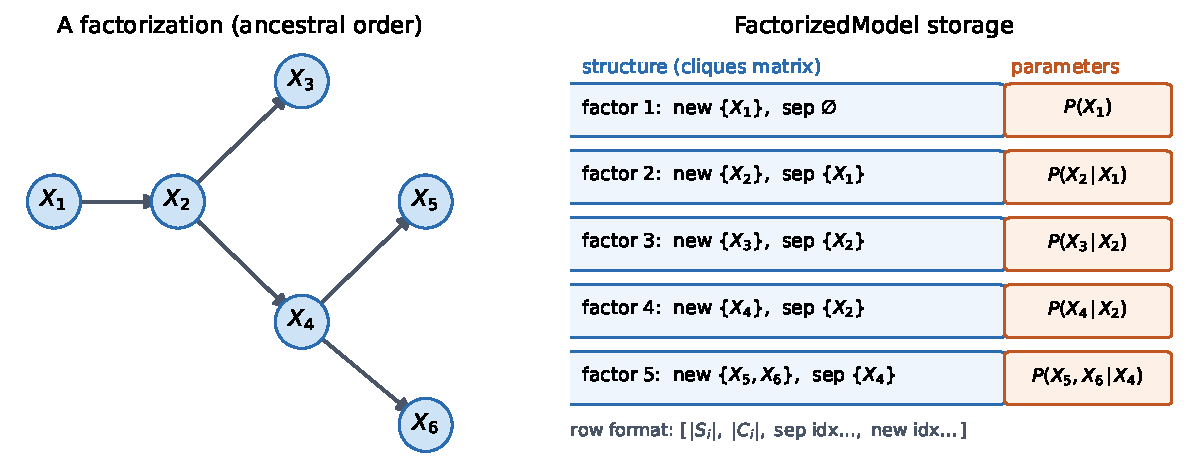
\includegraphics[width=\textwidth]{fig_factorization_storage.pdf}
\caption{How \texttt{pateda} stores an arbitrary ordered factorization. A
factorization over the variables (left) is kept as a cliques matrix
(\texttt{structure}, one row per factor giving its separator and new variables)
together with an aligned list of conditional probability tables
(\texttt{parameters}).}
\label{fig:factstorage}
\end{figure}

FDA (\texttt{FDA} class): when a user supplies a fixed clique structure (known from the problem domain), \texttt{LearnFDA} computes only the conditional probability tables from data, bypassing structure learning entirely.  This is the original factorized distribution algorithm of \citet{Muhlenbein_et_al:1999} where the structure of the interactions is not learned from data. 

\subsection{Univariate Models}
\label{sec:univariate}

Univariate models assume all variables are independent: $p(\mathbf{x}) = \prod_i p(x_i)$.  The marginal $p(x_i)$ is estimated as the empirical
frequency in the selected population (with optional Laplace smoothing $\alpha$).

\begin{description}
  \item[UMDA] \citep{Muhlenbein_and_Paas:1996}.
    Univariate marginal distribution algorithm.  Each marginal is learned independently from the selected population.
    Learning: \texttt{LearnUMDA}. Sampling: \texttt{SampleFDA}.

  \item[PBIL] \citep{Baluja:1994}.
    Population-based incremental learning.  Maintains a running estimate of the marginals updated with learning rate $\alpha$:
    $P^{(t+1)}(x_i) = (1 - \alpha)\,P^{(t)}(x_i) + \alpha\,\hat{P}(x_i)$.
    With $\alpha = 1$ PBIL reduces to UMDA.
    Learning: \texttt{LearnPBIL}. Sampling: \texttt{SampleFDA}.

  \item[MIMIC] \citep{DeBonet_et_al:1996}.
    Mutual Information Maximization for Input Clustering.
    Learns a chain-structured factorization that maximizes the sum of  pairwise mutual information along the chain.
    Learning: \texttt{LearnMIMIC}. Sampling: \texttt{SampleFDA}.
\end{description}

\subsection{Tree and Forest Models}
\label{sec:trees}

Tree-structured models represent pairwise variable dependencies using a maximum-weight spanning tree of the mutual-information matrix \citep{Chow_and_Liu:1968}.

\begin{description}
  \item[TreeEDA / Tree-EDA] \citep{Baluja_and_Davies:1997}.
    Learns a directed tree using Chow--Liu algorithm on pairwise MI.
    Learning: \texttt{LearnTreeModel}. Sampling: \texttt{SampleFDA}.

  \item[TreeEDAR / Tree-EDA\_r] \citep{Baluja:2006,Santana_et_al:2007b}
    Variant of Tree-EDA with a user-supplied \texttt{interaction\_matrix} that constrains which pairs of variables can form a dependency.
    Learning: \texttt{LearnTreeModelR}.

  \item[TreeEDAM / Tree-EDA-M] \citep{Santana_et_al:2005int}.
    Variant of Tree-EDA that keeps only \emph{malign} interactions.  For each pair of variables it compares the most probable joint configuration $\arg\max_{a,b} p(x_i=a,x_j=b)$ with the configuration that maximizes the product of the univariate marginals $(\arg\max_a p(x_i=a),\arg\max_b p(x_j=b))$.  If they coincide the interaction is \emph{benign} --- it only reinforces the main effects and can be reproduced by independent sampling --- so its mutual information is not computed and no edge is added.  Otherwise the interaction is \emph{malign} (deceptive) and is treated as in Tree-EDA.  The model is thus usually a forest, and reduces to UMDA when every interaction is benign.  The test is defined through $\arg\max$ of the marginal tables, so it applies unchanged to discrete non-binary variables.
    Learning: \texttt{LearnTreeModelM}. Sampling: \texttt{SampleFDA}.

  \item[Int\_FDA / Int-Tree] \citep{Santana_et_al:2002int}.
    Tree-based FDA for integer problems with \emph{very high cardinality}.  It uses the same Chow--Liu tree as Tree-EDA, but its model is \emph{not} a probability distribution: rather than storing a conditional table $P(X_j\mid X_i)$ of size $c\times c$ per edge, it stores the tree together with two index tables and the selected population itself.
    Column $i$ of \texttt{PopulValues} lists the indices of the selected vectors ordered by the value of $X_i$, and \texttt{ParentIndices} records, for each value, the boundaries of the corresponding block, so that ``pick a selected vector whose parent equals $v$'' is an $O(1)$ operation.
    Sampling copies genes from donor vectors along the tree: the root is copied from a random selected vector, and each child $X_j$ is copied from a random selected vector whose parent $X_i$ matches the value already assigned.  This reproduces the empirical tree distribution $p(x)=p(x_{root})\prod_i p(x_i\mid x_{pa(i)})$ \emph{exactly}, but needs only $O(N\cdot n + c\cdot n)$ memory instead of the $O(c^2\cdot n)$ of a table-based tree, which is what makes it practical when $c$ is large.
    Learning: \texttt{LearnIntFDA}. Sampling: \texttt{SampleIntFDA}.

  \item[BMDA] \citep{Pelikan_and_Muhlenbein:1999}
    Bivariate marginal distribution algorithm.  Detects pairwise dependencies with chi-square tests and builds a forest of bivariate conditionals.
    Learning: \texttt{LearnBMDA}.

  \item[AffEDA] \citep{Santana_et_al:2009c}.
    Affinity-propagation EDA 
    Uses affinity propagation on the MI matrix to discover variable cliques, then builds a factorized model over those cliques.
    Learning: \texttt{LearnAffinityFactorization}.

  \item[MTED / MT-EDA] \citep{Santana_et_al:2001br}.
    Mixture of trees EDA.  Learns $k$ tree components with mixture weights.
    Weight learning options: \texttt{"uniform"}, \texttt{"em"}, or \texttt{"fitness\_proportional"}.  Adaptive and prior-based extensions   are supported to prevent premature convergence.
    Learning: \texttt{LearnMixtureTrees}. Sampling: \texttt{SampleMixtureTrees}.
\end{description}

\subsection{Bayesian Network Models}
\label{sec:bayes}

Bayesian networks \citep{Lauritzen_and_Spiegelhalter:1988} are directed acyclic graphs in which $X_i$ is conditionally independent of its non-descendants given its parents $\mathbf{Pa}_i$.  The joint distribution factorizes as:

\begin{equation}
  p(\mathbf{x}) = \prod_{i=1}^{n} p(x_i \mid \mathbf{pa}_i).
\end{equation}

The local distribution $p(x_i \mid \mathbf{pa}_i)$ is a conditional probability table (CPT) with $r_i$ entries for each of the $q_i = \prod_{X_j \in \mathbf{Pa}_i} r_j$ parent configurations.

\begin{description}
  \item[EBNA] \citep{Etxeberria_and_Larranhaga:1999}.
    Estimation of Bayesian network algorithm.  Structure learning uses a greedy score-and-search procedure with the Bayesian information criterion (BIC) \citep{Schwarz:1978} or the Bayesian score  \citep{Cooper_and_Herskovits:1992}.
    Learning: \texttt{LearnEBNA}. Sampling: \texttt{SampleBayesianNetwork}.

  \item[BOA] \citep{Pelikan_et_al:1999,Pelikan:2005}.
    Bayesian optimization algorithm.  Greedy structure search with BIC/MDL scoring.
    Learning: \texttt{LearnBOA}. Sampling: \texttt{SampleBayesianNetwork}.

  \item[hBOA] \citep{Pelikan_and_Goldberg:2001,Pelikan:2005}.
    Hierarchical Bayesian optimization algorithm.  hBOA differs from BOA in the
    representation of the local conditional distributions: where BOA stores a full
    CPT with $q_i = \prod_{X_j \in \mathbf{Pa}_i} r_j$ rows, hBOA stores a decision
    tree or decision graph over the parents, so that only the parent configurations
    the data actually distinguishes receive their own parameters.  The number of
    parameters then grows with the complexity of the dependency rather than with
    $|\mathbf{Pa}_i|$, allowing hBOA to admit substantially larger parent sets than
    BOA at the same population size.  Decision graphs additionally \emph{merge}
    leaves, letting distinct parent configurations share parameters, which is what
    makes hBOA effective on hierarchically decomposable problems.  The complete
    algorithm of \citet{Pelikan:2005} also replaces generational replacement by
    restricted tournament replacement (RTR); as a replacement component this is
    orthogonal to the learning method and is configured separately in
    \texttt{EDAComponents}.
    Learning: \texttt{LearnHBOA}. Sampling: \texttt{SampleBayesianNetwork}.

  \item[LFDA] \citep{Muhlenbein_and_Mahnig:1999}.
    Learning factorized distribution algorithm.  Whereas FDA is given a
    factorization derived from the structure of an additively decomposable
    function, LFDA learns a Bayesian network from the selected population at each
    generation and uses it as the factorization.  Structure search is greedy
    hill-climbing on a BIC score whose complexity penalty carries a weighting
    factor $\alpha$,
    $\mathrm{BIC}(B,D,\alpha) = \sum_i \log P(D_i \mid \mathbf{Pa}_i, \theta_{ML})
    - \alpha \frac{\log N}{2} |\theta|$,
    subject to a hard bound $k$ on the number of parents per variable.  Increasing
    $\alpha$ yields sparser networks and is the principal control on overfitting
    given the small samples available inside an EDA.
    Learning: \texttt{LearnLFDA}. Sampling: \texttt{SampleBayesianNetwork}.

  \item[PADA] \citep{Soto_et_al:1999,Ochoa_et_al:2000}.
    Polytree approximation of distribution algorithm.  PADA restricts the model to
    a \emph{polytree}, a singly connected Bayesian network whose undirected
    skeleton contains no loops.  Unlike the score-and-search algorithms above,
    PADA learns the structure with independence tests: the LPA algorithm builds a
    candidate edge list from marginal dependencies $\mathrm{Dep}(a,b) > e_0$,
    discards pairs explained away by a third variable
    ($\mathrm{Dep}(a,b \mid c) < e_1$), ranks the survivors by the global
    dependency degree, inserts edges while keeping the skeleton singly connected,
    and orients head-to-head nodes using the fact that conditioning on a collider
    \emph{raises} the dependency between its parents.  A polytree has at most $n-1$
    edges, so its parameters remain estimable from small populations, while still
    admitting multiple parents and colliders that a tree model cannot express.
    Learning: \texttt{LearnPADA}. Sampling: \texttt{SampleBayesianNetwork}.
\end{description}

\subsection{Most Probable Configurations}
\label{sec:mpe}

Both EBNA and BOA sample new individuals using probabilistic logic sampling over the directed network. Beyond random sampling, \texttt{pateda} can also generate the \emph{deterministic} high-probability configurations of a learned model. This is motivated by the observation that, especially in late generations, the mode of the model is often a very good (sometimes the optimal) solution, and that inspecting several modes reveals the multiple basins the model has captured \citep{Echegoyen_et_al:2007}.

The single \emph{most probable explanation} (MPE) is the configuration
$\mathbf{x}^\ast = \arg\max_{\mathbf{x}} p(\mathbf{x})$. More generally, the
\emph{$k$ most probable configurations} ($k$-MPC / $k$-MAP) are the $k$ highest-probability
configurations, which \texttt{pateda} computes exactly, per model type, rather than by
enumeration:

\begin{description}
  \item[Univariate models] \texttt{KMPCUnivariate} uses Nilsson's partition
    scheme: the top configuration is the per-variable mode, and the next best
    ones are obtained by the cheapest single-variable substitutions.
  \item[Tree / junction-tree / factorized models]
    \texttt{KMPCTree} and \texttt{KMPCJunctionTree} run max-product (max-sum in
    log space) message passing followed by Nilsson's most-probable-flip
    backtracking to enumerate the ordered list of configurations.
  \item[Bayesian networks] \texttt{KMPCBayesianNetwork} performs the same
    $k$-MAP over the CPD factorization of an EBNA/BOA network.
  \item[Markov networks] the engine in
    \texttt{inference/map\_inference.py} provides the single MPE by exact
    junction-tree inference, max-product belief propagation, decimation
    (iteratively fixing the most certain variable), or a greedy fallback.
\end{description}

The dispatcher \texttt{compute\_kmpc(model, cardinality, k)} selects the right
algorithm automatically from the model type and returns a \texttt{KMPCResult}
with the configurations and their (log-)probabilities; \texttt{compute\_map}
returns just the MPE. These can be used as a sampler that injects the model's
modes into the new population, or as an analysis tool after a run.

\subsection{Markov Network Models}
\label{sec:markov}

A Markov random field (MRF) \citep{Hammersley_and_Clifford:1968} is an undirected graphical model in which the joint distribution factorizes over the cliques of the graph as a Gibbs distribution:

\begin{equation}
  p(\mathbf{x}) = \frac{1}{Z}\exp\!\left(-H(\mathbf{x})\right),\quad
  H(\mathbf{x}) = \sum_{C \in \mathcal{C}} \Phi_C(\mathbf{x}_C)
\end{equation}

where $\mathcal{C}$ is the set of maximal cliques and $Z$ is the partition function.  Sampling from MRFs typically uses Gibbs sampling: iteratively sample each variable $X_i$ from its conditional distribution given the current values of its neighbors $N(X_i)$.

\begin{description}
  \item[MN-FDA / MNFDA] \citep{Santana:2003c}.
    Detects pairwise dependencies with a $\chi^2$ independence test, extracts the
    maximal cliques of the resulting dependency graph, and turns them into an
    ordered factorized model (junction graph). The model can be sampled with PLS
    (\texttt{SampleFDA}, recommended for small cliques) or Gibbs sampling.
    Learning: \texttt{LearnMNFDA}. Sampling: \texttt{SampleFDA}.

  \item[MN-FDA\_r / MNFDAR] \citep{Santana:2005}.
    MN-FDA \emph{restricted} to a known interaction structure: dependency testing
    is performed only for the variable pairs allowed by a binary interaction
    matrix $R$, so the learned network is a subgraph of the unrestricted MN-FDA
    network consistent with the a-priori problem structure (Section~\ref{sec:apriori}).
    Learning: \texttt{LearnMNFDAR}. Sampling: \texttt{SampleFDA}.

  \item[MN-FDAg / MNFDAG] \citep{Santana:2005}.
    Identical pipeline to MN-FDA but using the \emph{$G$-test} of independence
    ($G(X_i,X_j)=2N\cdot\mathrm{MI}(X_i,X_j)$, with
    $\mathrm{df}=(r_i-1)(r_j-1)$) instead of the $\chi^2$ threshold. The $G$-test
    is a more principled likelihood-ratio criterion and behaves better for
    variables of differing cardinality.
    Learning: \texttt{LearnMNFDAG}. Sampling: \texttt{SampleFDA} or \texttt{SampleGibbs}.

  \item[MN-FDAg\_r / MNFDAGR] \citep{Santana:2005}.
    MN-FDAg \emph{restricted} to a known interaction matrix $R$, the $G$-test
    counterpart of MN-FDA\_r.
    Learning: \texttt{LearnMNFDAGR}. Sampling: \texttt{SampleFDA} or \texttt{SampleGibbs}.

  \item[MOA] \citep{Shakya_and_McCall:2007,Shakya_and_Santana:2008}.
    Markovianity-based optimization algorithm.  Learns local $k$-neighborhoods for each variable and samples via Gibbs sampling.
    Learning: \texttt{LearnMOA}. Sampling: \texttt{SampleGibbs}.
\end{description}

The four MN-FDA variants therefore differ along only \emph{two} orthogonal axes,
and are best understood as a $2\times2$ table rather than four unrelated methods:
the \emph{dependency test} used to decide which edges enter the Markov network
($\chi^2$ for MN-FDA/MN-FDA\_r vs. the $G$-test for MN-FDAg/MN-FDAg\_r), and
whether structure learning is \emph{unrestricted} (MN-FDA, MN-FDAg) or
\emph{restricted} to an a-priori interaction matrix $R$ (the ``\_r'' variants).
The downstream representation (an ordered factorized/junction-graph model) and
the available samplers (PLS or Gibbs) are shared by all four.

\subsection{Markov Chain Models}
\label{sec:markov_chain}

\begin{description}
  \item[MK-EDA / MKEDA] \citep{Santana_et_al:2004}.
    $k$-order Markov chain EDA.  Each variable $X_i$ depends on the $k$
    preceding variables in a fixed linear ordering:
    $p(\mathbf{x}) = p(x_1)\prod_{i=2}^{n} p(x_i \mid x_{i-k}, \ldots, x_{i-1})$.
    Well-suited to problems with a natural sequential structure (e.g. protein folding with relative encodings).
    Learning: \texttt{LearnMarkovChain}. Sampling: \texttt{SampleMarkovChain}.

  \item[MkRg-EDA] \citep{Santana_et_al:2011reg}.
    Regularized $k$-order Markov EDA.  It keeps the $k$-order Markov structure of MK-EDA but replaces each conditional probability table --- whose size is exponential in $k$ --- by a \emph{regularized multinomial logistic regression} that predicts $X_i$ from (a function of) its previous $k$ variables, fitted with the elastic net \citep{Zou_and_Hastie:2005}.  This keeps the number of parameters polynomial in $k$, so larger orders become affordable, and the regularization prunes the previous variables that do not contribute.  Three predictor variants of increasing complexity are available through the \texttt{variant} argument: \texttt{"rgk"} (the $k$ previous variables, $O(k)$ parameters), \texttt{"bivrgk"} (their pairwise products, $O(k^2)$) and \texttt{"allrgk"} (both, $O(k^2)$).  Sampling generates the variables in order, seeding the first $k$ from the selected population and drawing each remaining variable from its regressed conditional distribution.
    Learning: \texttt{LearnRegularizedMarkov}. Sampling: \texttt{SampleRegularizedMarkov}.
\end{description}

\subsection{Constrained EDAs}
\label{sec:constrained}

\begin{description}
  \item[CUMDA] \citep{Santana_and_Ochoa:1999b}.
    Unitation-constrained UMDA.  Every solution must contain exactly \texttt{n\_ones} ones.  The seeding method
    (\texttt{SeedingUnitationConstraint}) generates feasible initial solutions, and the sampling method (\texttt{SampleCUMDA}) uses
    Stochastic Universal Sampling to maintain the constraint.
    Learning: \texttt{LearnCUMDA}.

  \item[CFDA] \citep{Santana_et_al:2001c}.
    Unitation-constrained FDA.  Uses a tree-structured factorized model while enforcing the same fixed-unitation constraint as CUMDA.
    Learning: \texttt{LearnCFDA}. Sampling: \texttt{SampleCFDA}.
\end{description}

\subsection{Continuous Gaussian Models}
\label{sec:gaussian}

While \texttt{pateda} includes several continuous-based EDAs, these methods have not been tested, enhanced, and extended to the same extent as the discrete implementations. Other Python libraries implement more comprehensive approaches to the optimization of continuous problems with model-based evolutionary algorithms: the CMA-ES family \cite{Nomura_and_Shibata:2019} and, closest in spirit to \texttt{pateda}, the \texttt{EDAspy} package \citep{Soloviev_et_al:2024}, which provides a range of univariate, multivariate-Gaussian and copula-based continuous EDAs. Users targeting continuous optimization are encouraged to consider these libraries alongside \texttt{pateda}.

\begin{description}
  \item[\textbf{GaussianUMDA}] \citep{Larranhaga_et_al:1999,Larranhaga_et_al:2000}.
    Each variable is modeled independently as a Gaussian:
    $p(x_i) = \mathcal{N}(x_i; \mu_i, \sigma_i^2)$.
    Parameters $(\mu_i, \sigma_i^2)$ are estimated from the selected population.
    Learning: \texttt{LearnGaussianUnivariate}. Sampling: \texttt{SampleGaussianUnivariate}.

  \item[\textbf{GaussianFull}] \citep{Larranhaga_et_al:2000,Bosman_and_Thierens:2000}.
    Full multivariate Gaussian: $p(\mathbf{x}) = \mathcal{N}(\mathbf{x};\boldsymbol{\mu},\Sigma)$.
    All pairwise dependencies are captured by the covariance matrix $\Sigma$.
    May suffer from variance collapse in later generations\citep{Bosman_and_Grahl:2008}; a variance scaling parameter is provided.
    Learning: \texttt{LearnGaussianFull}. Sampling: \texttt{SampleGaussianFull}.

  \item[\textbf{GaussianNetworkEDA}]
    Gaussian network (GMRF) EDA.  Learns a sparse Gaussian graphical model where each variable's local distribution is a linear regression on its parents in a directed graph.  The GMRF approach identifies relevant conditional independences in continuous data.

  \item[\textbf{MixtureGaussianEDA}] \citep{Bosman_and_Thierens:2002}.
    Mixture of Gaussian distributions.  The population is first clustered  (k-means or similar), then a separate Gaussian (univariate or full) is fit to each cluster.  Suitable for multimodal search landscapes.
    Learning: \texttt{LearnMixtureGaussian}. Sampling: \texttt{SampleMixtureGaussian}.
\end{description}

\subsection{Learning from Weighted Solutions}
\label{sec:weighted_learning}

All the learners above estimate their model from the selected set by treating
every selected solution equally. \texttt{pateda} generalizes this by letting each
selected individual carry a \emph{weight} that scales its contribution to the
sufficient statistics (counts, mutual information, covariances) of \emph{any}
model. This blends structure/parameter learning with fitness guidance without
changing the learner: a weight of $1$ for every individual recovers the classic
EDA, while fitness-dependent weights let better solutions influence the model
more. The behaviour is controlled by the \texttt{selection\_weighting} argument of
the \texttt{EDA} constructor:

\begin{lstlisting}
eda = EDA(pop_size, n_vars, fitness_func, cardinality,
          components,
          selection_weighting="boltzmann",   # "uniform" | "proportional" | "boltzmann"
          weighting_beta=2.0)   # higher beta -> stronger fitness pressure
\end{lstlisting}

\texttt{"uniform"} is the classic EDA; \texttt{"proportional"} weights each
selected solution by its (normalized) fitness; \texttt{"boltzmann"} weights it by
$e^{\beta f(\mathbf{x})}$. This subsumes as a special case the older
fitness-weighted univariate scheme (the ``Bisection''/BSC method of
\citet{Inza_et_al:2000}), which is exactly a univariate learner run with
proportional weighting; for this reason BSC is no longer provided as a separate
algorithm class. Because the weighting acts at the sufficient-statistic level it
composes with every model family --- univariate, tree, Bayesian network, Markov
network, factorized, and Gaussian alike.

%% ============================================================
\section{EDA Components}
\label{sec:components}
%% ============================================================

\subsection{Seeding Methods}

Seeding methods initialize the population at generation 0. In an EDA the seed
matters more than in a genetic algorithm: it is the only sample the very first
model is estimated from, so a biased or infeasible seed directly biases the
first learned distribution. Seeding is therefore also the natural entry point
for a-priori knowledge (biased marginals, feasibility constraints, or a
warm-start population from a previous run; Sections~\ref{sec:apriori}
and~\ref{sec:transfer}).

\begin{description}
  \item[\texttt{RandomInit}]
    Samples each variable uniformly from its range.
    For discrete variables: integer in $[0, r_i)$.
    For continuous variables: real in $[\ell_i, u_i]$.

  \item[\texttt{BiasInit}]
    Biased binary initialization.  Variable $X_i$ is set to 1 with probability
    $p$ and to 0 with probability $1-p$.

  \item[\texttt{ProbabilisticInit}]
    Generalizes \texttt{BiasInit} to arbitrary discrete variables: each variable
    is sampled from a user-supplied categorical distribution over its
    \texttt{cardinality} values, so the initial population follows a chosen
    product distribution $\prod_i P(X_i)$. It is the natural way to seed a
    non-binary problem with per-configuration prior beliefs (a form of a-priori
    knowledge; \texttt{BiasInit} is the binary special case).

  \item[\texttt{SeedingUnitationConstraint}]
    Generates binary solutions with exactly \texttt{num\_ones} ones.
    Required by \texttt{CUMDA} and \texttt{CFDA}.

  \item[\texttt{SeedThisPop}]
    Uses a user-supplied population as generation~0 instead of generating one.
    The population is passed at run time through the \texttt{initial\_population}
    parameter (an array of shape \texttt{(pop\_size, n\_vars)}); the method
    validates its shape and returns it unchanged. This is the mechanism used to
    warm-start a run from the output of a previous EDA.
\end{description}

\subsection{Selection Methods}

Selection determines which individuals are used for model learning. This is the
single most consequential component of an EDA: it defines the empirical
distribution the model is fitted to, and hence the search bias. Whereas in a
genetic algorithm selection only decides who reproduces, in an EDA it decides
\emph{what is modelled} --- stronger selection sharpens the target distribution
but risks collapsing diversity and inducing spurious dependencies from a small,
skewed selected set. The role of selection in EDAs has been studied by
\citet{Johnson_and_Shapiro:2002,Lima_et_al:2007,Mahnig_and_Muehlenbein:2001,Santana_et_al:2005b}.

\begin{description}
  \item[\texttt{TruncationSelection}]
    Selects the top $\lfloor \texttt{ratio} \cdot N \rfloor$ individuals by
    fitness.  This is the most common selection method in EDAs.

  \item[\texttt{TournamentSelection}]
    Tournament selection of configurable size.

  \item[\texttt{ProportionalSelection} / \texttt{SUSSelection}]
    Fitness-proportional selection using stochastic universal sampling (SUS)
    \citep{Baker:1987}.

  \item[\texttt{BoltzmannSelection}]
    Selection with Boltzmann temperature; probability proportional to
    $e^{\beta f(x)}$.

  \item[\texttt{RankingSelection}]
    Rank-based selection; probability proportional to $2r/(N(N+1))$ where
    $r$ is the fitness rank.

  \item[\texttt{NonDominatedSelection}]
    Selects the non-dominated front.  For multi-objective problems.

  \item[\texttt{CrowdingSelection}]
    NSGA-II-style: non-dominated sorting + crowding distance tie-breaking.

  \item[\texttt{IndicatorBasedSelection}]
    SMS-EMOA-style hypervolume indicator-based selection.

  \item[\texttt{ParetoFrontSelection}]
    Selects complete Pareto fronts up to the selection quota.
\end{description}

\subsection{Replacement Methods}

Replacement decides which solutions survive into the next generation and thus
controls the population's turnover. In EDAs the default is full generational
replacement, because each generation is meant to be a fresh sample from the
current model; elitism is nonetheless useful to avoid losing the best solution
when the model drifts. Replacement is also where \emph{diversity-preserving}
schemes (crowding, restricted tournament, clustering) belong --- they let an EDA
maintain several basins at once, which is important on multimodal problems and
is the mechanism the complete hBOA relies on (Section~\ref{sec:bayes}).

\begin{description}
  \item[\texttt{ElitistReplacement}]
    Copies the best \texttt{n\_elite} solutions from the previous generation
    into the new population if they are better than the worst new individual.
    When \texttt{n\_elite} is left unset the number of elites defaults to
    \texttt{elite\_ratio}~$=0.1$ of the population; the plug-and-play algorithm
    classes instead instantiate it with \texttt{n\_elite}~$=1$ (preserve the
    single best) when \texttt{elitism=True}.

  \item[\texttt{GenerationalReplacement}]
    New population completely replaces the old one.

  \item[\texttt{DeterministicCrowdingReplacement}] \citep{Mahfoud:1995}.
    Deterministic crowding: each new individual competes with the \emph{most
    similar} current individual (Hamming distance for discrete, Euclidean for
    continuous) and replaces it only if at least as fit, so distinct niches
    survive.

  \item[\texttt{RestrictedTournamentReplacement}] \citep{Harik:1995}.
    Restricted tournament replacement (RTR): each new individual competes with
    the most similar member of a random window of size \texttt{window\_size};
    the complete hBOA (Section~\ref{sec:bayes}) relies on this scheme.

  \item[\texttt{ClusteringReplacement}].
    The merged population is clustered (k-means) and elitism is applied
    \emph{within} each cluster, with a per-cluster quota proportional to the
    cluster size, preserving one niche per cluster.
\end{description}

The three diversity-preserving schemes share the \texttt{ReplacementMethod}
interface, so they can be dropped into any pipeline and are useful on multimodal
problems where plain elitism would collapse the population onto one basin.

\subsection{Stopping Conditions}

A stopping condition ends the generational loop. Besides the usual budget and
target-value criteria, EDAs admit a natural model-based stopping signal: once the
learned distribution has converged (marginals near $0/1$, population diversity
near zero) further sampling cannot escape the current basin, so detecting
convergence avoids wasting evaluations.

\begin{description}
  \item[\texttt{MaxGenerations}]
    Stops after a fixed number of generations.

  \item[\texttt{MaxGenerationsOrOptimum}]
    Stops when either the generation limit is reached or a known optimal fitness
    value (passed as \texttt{optimal\_fitness}) is attained.

  \item[\texttt{NoImprovement}]
    Stagnation test: stops when the best fitness has not improved by more than
    \texttt{epsilon} over the last \texttt{k} generations.

  \item[\texttt{PopulationConvergence}]
    Stops when the population diversity drops below \texttt{tol} (mean
    per-variable value agreement for discrete populations, relative dispersion
    for continuous ones), optionally requiring the condition to persist for a
    \texttt{patience} of generations.

  \item[\texttt{CompositeStop}]
    Combines several conditions with an \texttt{"any"} (stop when the first
    fires) or \texttt{"all"} rule, e.g. a hard generation cap together with a
    stagnation or convergence test.
\end{description}

\subsection{Local Optimization}

Local optimization turns an EDA into a \emph{memetic} algorithm: sampled
solutions are refined by a local search before selection. This is especially
effective for EDAs, because polishing solutions sharpens the statistical signal
the model learns from --- building blocks are completed, so the dependencies
between their variables become easier to detect --- while the global model
supplies the diversification the local search lacks. The two operators of
Section~\ref{sec:structure_exploitation} go one step further and localize the
search using the model's own structure.

\begin{description}
  \item[\texttt{GreedySearch}]
    Greedy hill climbing in the continuous case.

  \item[\texttt{DiscreteGreedySearch}]
    Greedy flip-based local search for discrete problems.

  \item[\texttt{DiscreteSimulatedAnnealing}]
    Simulated annealing for discrete problems.

  \item[\texttt{ContiguousBlockOptimization}]
    Specialized local search for contiguous-block problems.

  \item[\texttt{ScipyLocalSearch}]
    Wraps \texttt{scipy.optimize.minimize} for continuous local optimization.
    Any \texttt{scipy} method can be selected (e.g. \texttt{"L-BFGS-B"},
    \texttt{"Nelder-Mead"}, \texttt{"Powell"}, \texttt{"CG"}), with a per-solution
    iteration and function-evaluation cap.
\end{description}

For continuous problems, combining a Gaussian EDA with different \texttt{scipy}
local searches is a one-line change of the \texttt{method} argument:

\begin{lstlisting}
from pateda.local_optimization.scipy_local_search import ScipyLocalSearch
# gradient-based refinement of the sampled solutions
local = ScipyLocalSearch(method="L-BFGS-B", max_iter=100, max_fun_evals=200)
# ... pass local as EDAComponents(local_optimization=local, ...)
\end{lstlisting}

A worked comparison of several \texttt{scipy} methods inside a Gaussian EDA on
Rastrigin is provided in \texttt{examples/continuous\_memetic\_eda.py}, where
Powell's method drives the EDA to the global optimum that the plain EDA does not
reach.

\subsubsection{Budget- and subset-aware memetic local search}
\label{sec:budgeted_ls}

A family of discrete local optimizers designed to be used as the local-search
step of a memetic EDA: after sampling, they are applied to a \emph{subset} of the
population under a shared \emph{evaluation budget}.  All of them share one
interface --- the base class \texttt{BudgetedLocalSearch} --- so they are fully
interchangeable in a pipeline.  Two parameters, common to every optimizer,
control the local-search intensity: \texttt{subset\_fraction} (the fraction of
sampled solutions the search is applied to, selected as the best, a random
subset, or the worst) and \texttt{evaluation\_budget} (the total number of
fitness evaluations spent per generation, shared equally among the selected
solutions).  A neighbor changes one variable to another value of its domain, so
the optimizers work for binary and non-binary discrete variables alike.

\begin{description}
  \item[\texttt{DeterministicHillClimber}] \citep{Radetic_et_al:2009}.
    Steepest-ascent single-change hill climber (the deterministic hill climber,
    DHC): the whole single-change neighborhood is evaluated and the
    best-improving move applied, until a local optimum is reached.

  \item[\texttt{FirstImprovementHillClimber}] \citep{Hansen_and_Mladenovic:2003}.
    First-improvement descent: neighbors are scanned in random order and the
    first improving move is applied.

  \item[\texttt{StochasticHillClimber}].
    Random-mutation hill climbing (RMHC): a single random change is proposed
    each step and accepted iff it does not worsen the fitness.

  \item[\texttt{SimulatedAnnealing}] \citep{Kirkpatrick_et_al:1983}.
    Metropolis simulated annealing over the single-change neighborhood, with
    geometric or linear cooling stretched over the evaluation budget and an
    optional automatic initial temperature.

  \item[\texttt{VariableNeighborhoodSearch}] \citep{Hansen_and_Mladenovic:2003}.
    Basic VNS: shake the incumbent in the growing $k$-th (Hamming distance $k$)
    neighborhood, run a local descent, and keep the result only if it improves,
    otherwise widen the shake.

  \item[\texttt{ReducedVariableNeighborhoodSearch}] \citep{Hansen_and_Mladenovic:2003}.
    Reduced VNS: the same neighborhood-change scheme without the descent, for
    problems where evaluations are expensive.
\end{description}

\subsection{Exploiting the model structure: network crossover and substructural search}
\label{sec:structure_exploitation}

Most samplers in pateda draw new solutions from the \emph{probabilities} of the learned model (probabilistic logic sampling, Gibbs sampling, most-probable configurations).  The graphical \emph{structure} of the model can also be exploited directly, in two ways that do not use its probabilities at all.  Both are generic: a learned model of any class (Bayesian network, tree, factorized or Markov-network model) is mapped to a graph view by \texttt{model\_to\_linkage\_graph} / \texttt{model\_to\_substructures} in \texttt{knowledge\_extraction}, and the very same operators also accept a linkage graph known a priori from the problem (an additive function's blocks, an Ising lattice, a UBQP weight matrix, a SAT clause graph).

\begin{description}
  \item[\texttt{SampleNetworkCrossover}] \citep{Hauschild_and_Pelikan:2010}.
    Network crossover: a recombination operator (implemented as a \texttt{SamplingMethod}, with the population supplied as the parent pool).  It grows a \emph{connected} crossover mask on the linkage graph --- by randomized breadth-first search (\texttt{"bfs"}) or a random walk (\texttt{"random\_walk"}) --- and swaps the masked variables between two parents.  Because the mask is connected, its boundary cuts the \emph{weakest} dependencies, so tightly-linked building blocks are inherited together and not disrupted.  It is the structural analogue of the crossover operators in \texttt{pateda.crossover}, and the recombination counterpart of the partial samplers: partial sampling \emph{resamples} a subset of variables from the model, network crossover \emph{swaps} a connected subset between parents.

  \item[\texttt{SubstructuralLocalSearch}] \citep{Lima_et_al:2006}.
    Substructural neighborhood search: a local search (a \texttt{LocalOptMethod} subclassing \texttt{BudgetedLocalSearch}, so it shares the \texttt{subset\_fraction} / \texttt{evaluation\_budget} intensity controls) that hill-climbs over the joint values of whole \emph{substructures} rather than single variables.  For a Bayesian network the substructure of $X_i$ is $\{X_i\}\cup\mathbf{Pa}_i$ (\texttt{"parental"}), $\{X_i\}\cup\Omega_i$ (\texttt{"children"}) or their union (\texttt{"both"}); for a factorized / Markov model it is a clique (\texttt{"clique"}); a generic Markov-blanket neighborhood (\texttt{"neighborhood"}) is also available.  Each substructure's $\prod_{i\in S} r_i$ value combinations are enumerated and the best-improving one is accepted using the actual fitness.  Optimizing a linkage group as a unit escapes the deception that traps a single-variable hill climber, providing the intensification that complements the model-based global search.  The EDA passes the current model to the local search automatically.
\end{description}

The two operators express the rationale of exploiting the learned structure in complementary ways: network crossover recombines while \emph{avoiding model disruption}, and substructural search \emph{intensifies} the search within the model's linkage groups.

\subsection{Crossover and Mutation as Learning and Sampling}
\label{sec:crossover_as_model}

A useful consequence of the learning/sampling decomposition at the heart of
\texttt{pateda} is that classical genetic operators fit the same interface: a
recombination or mutation operator can be expressed as a (non-probabilistic)
\emph{learning} step that records how offspring will be produced, followed by a
\emph{sampling} step that produces them. The ``model'' is then simply the
procedural description of the operator rather than a probability distribution.
This is the \emph{non-probabilistic model} paradigm of MATEDA-2.0, and it lets
crossover and mutation be dropped into a pipeline, combined with model operators,
and searched over by the grammar (Section~\ref{sec:pipelines}) on an equal
footing with UMDA, EBNA, and the rest.

Concretely, \texttt{pateda} implements the classic \emph{two-point crossover}
this way. Its learning phase (\texttt{LearnTwoPointCrossover}) pairs up the
selected solutions and, for each pair, draws two cut points, storing the pairs
and cut points in the model; its sampling phase
(\texttt{SampleTwoPointCrossover}) applies those cuts to generate the offspring,
optionally followed by a mutation operator. The same recipe yields
\texttt{Learn}/\texttt{SampleBlockCrossover} (block/uniform-style exchange) and
\texttt{Learn}/\texttt{SampleTransposition} (a permutation-style transposition
operator); mutation operators such as \texttt{RandomResetMutation} plug into the
\texttt{mutation} slot of \texttt{EDAComponents}. Any further crossover operator
can be added by following the same two-phase split: store the procedure when
learning, execute it when sampling.

\subsection{Repairing Methods}

\begin{description}
  \item[\texttt{BoundsRepair}]
    Clips continuous variable values to their feasible bounds.

  \item[\texttt{TrigonometricRepair}]
    Trigonometric projection for angular variables.

  \item[\texttt{UnitationRepair}]
    Adjusts binary solutions to satisfy a fixed unitation constraint.
\end{description}

%% ============================================================
\section{Test Functions and Benchmark Problems}
\label{sec:functions}
%% ============================================================

The benchmark suite is organized by \emph{representation} and by \emph{kind}
inside the \texttt{functions/} package, so that the intended cardinality of a
problem and whether it is an academic toy or a combinatorial problem are explicit
from its location:

\begin{center}
\begin{tabular}{lp{9.2cm}}
\toprule
\textbf{Group} & \textbf{Contents} \\
\midrule
\texttt{discrete\_binary/toy\_functions/} & Pseudo-Boolean academic benchmarks: OneMax, trap/deceptive, NK landscapes, contiguous-block functions. \\
\texttt{discrete\_binary/problems/} & Binary combinatorial problems: Ising, UBQP, SAT, HP protein folding, max-clique and other graph problems. \\
\texttt{discrete\_non\_binary/toy\_functions/} & Integer / categorical benchmark functions (multi-valued deceptive, etc.). \\
\texttt{discrete\_non\_binary/problems/} & Non-binary combinatorial problems (e.g. graph colouring, Braid). \\
\texttt{continuous/toy\_functions/} & Real-valued benchmarks: Sphere, Rastrigin, Rosenbrock, Ackley, Griewank. \\
\texttt{continuous/problems/} & Continuous problems: AB off-lattice protein model, GNBG instances. \\
\bottomrule
\end{tabular}
\end{center}

Shared readers for graph-instance files live in \texttt{functions/graph\_utils.py}
and serve both the binary and non-binary graph problems. Figure~\ref{fig:probstruct}
illustrates the interaction structure that characterizes several of these
problems --- the very structure a good EDA is expected to recover in its model.

\begin{figure}[ht]
\centering
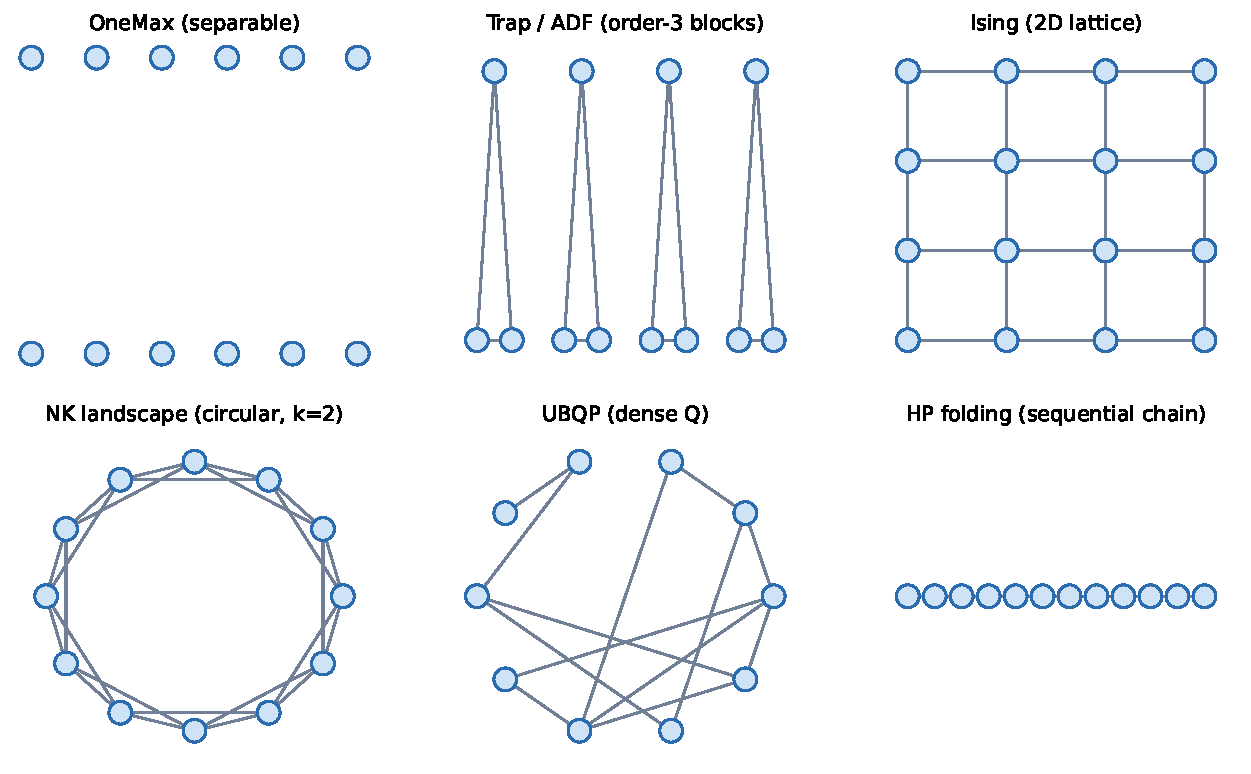
\includegraphics[width=\textwidth]{fig_problem_structures.pdf}
\caption{Variable-interaction structure of representative benchmark problems.
Separable problems (OneMax) have no edges; additively decomposable / trap
functions decompose into disjoint blocks; the Ising model is a lattice; NK
landscapes use a (here circular) neighborhood; UBQP has a dense interaction
matrix; and the HP folding model has a sequential chain structure. References:
trap/deceptive \citep{Ackley:1987,Goldberg:1987}, NK \citep{Kauffman:1993}, HP
\citep{Dill:1985}, SAT \citep{Selman_et_al:1992}.}
\label{fig:probstruct}
\end{figure}

\subsection{Discrete Functions}

\begin{description}
  \item[\textbf{OneMax}] Maximizes $f(\mathbf{x}) = \sum_i x_i$.
    The simplest EDA benchmark; all variables are independent.

  \item[\textbf{Trap functions}] Deceptive order-$k$ subfunctions
    \citep{Ackley:1987}:
    $f(\mathbf{x}) = \sum_{j} \text{trap}_k(u_j)$ where $u_j$ is the
    number of ones in block $j$.  Optimal solution is the all-ones string;
    the deceptive attractor is the all-zeros string.

  \item[\textbf{Deceptive functions}] Goldberg's deceptive functions
    \citep{Goldberg:1987}.

  \item[\textbf{Additively decomposable functions (ADFs)}]
    $f(\mathbf{x}) = \sum_i f_i(\mathbf{x}_{S_i})$ where each subfunction
    $f_i$ is defined over a disjoint subset $S_i$ of variables.  Ideal for
    studying the structural identification capabilities of EDAs.

  \item[\textbf{NK landscapes}] \citep{Kauffman:1993}.
    Each variable depends on $k$ others drawn uniformly or in circular topology.
    The subfunction value for each configuration is drawn at random.

  \item[\textbf{Ising model}]
    Energy minimization on a lattice:
    $E = -\sum_{i<j} J_{ij}\sigma_i\sigma_j - \sum_i h_i\sigma_i$.

  \item[\textbf{HP protein folding}] \citep{Dill:1985}.
    2-D/3-D lattice model.  Solutions encode the sequence of relative moves of
    amino acid residues.  pateda uses the relative encoding with a backtracking
    repair heuristic.

  \item[\textbf{SAT}] \citep{Selman_et_al:1992}.
    Satisfiability problems; single- and multi-objective versions available.

  \item[\textbf{UBQP}]
    Unconstrained binary quadratic programming:
    $f(\mathbf{x}) = \mathbf{x}^T Q \mathbf{x}$.

  \item[\textbf{Contiguous-block functions}]
    Reward solutions with long contiguous blocks of identical bits.

  \item[\textbf{Integer functions}]
    Functions over multi-valued (non-binary) discrete variables.
\end{description}

\subsection{Continuous Functions}

\begin{description}
  \item[\textbf{Standard benchmarks}] (\texttt{functions/continuous/benchmarks.py}):
    Sphere, Rastrigin, Rosenbrock, Ackley, Griewank.

  \item[\textbf{AB off-lattice protein model}] \citep{Larranhaga_et_al:1999}.
    Off-lattice protein model with Lennard-Jones interactions.
    Variables are bond angles in $[0, 2\pi]$.

  \item[\textbf{GNBG instances}] \citep{Yazdani_et_al:2023}
    Generalized numerical benchmark generator instances
    (\texttt{GNBG\_Instances.Python-main/}).
\end{description}

\texttt{pateda} includes examples on how to test EDA implementations on discrete benchmarks such as the PBO suite \cite{Doerr_et_al:2019} through linking with different Python libraries of the Iterative Optimization Heuristics ecosystem \cite{Vermetten_et_al:2024}. Examples on how to link to the   Generalized Numerical Benchmark Generator (GNBG) of continuous functions\citep{Yazdani_et_al:2023} are also included.

%% ============================================================
\section{Multi-Objective Optimization}
\label{sec:multiobjective}
%% ============================================================

\subsection{Multi-Objective Problem Definition}

A multi-objective optimization problem (MOP) \citep{Deb:2001} requires simultaneously optimizing $m$ objectives $f_1(\mathbf{x}), \ldots, f_m(\mathbf{x})$. Since objectives usually conflict, the goal is to find the \emph{Pareto front}: the set of non-dominated solutions where no single objective can be improved without degrading another.

While \texttt{pateda} is not a specialized library for solving multi-objective problems, it addresses these problems by modifying the selection scheme in such a way that different multi-objective approaches are indirectly implement.

For multi-objective problems, the objective function is suppossed to return a vector of $m$ values: 

\begin{lstlisting}
def bi_objective(x):
    f1 = np.sum(x)            # first objective (maximise)
    f2 = -np.sum((x - 0.5)**2)  # second objective (maximise)
    return np.array([f1, f2])
\end{lstlisting}

\subsection{Pareto Dominance}

\texttt{pateda} implements Pareto dominance in \texttt{multiobjective/dominance.py}. Solution $\mathbf{x}$ dominates $\mathbf{y}$ if it is at least as good on all objectives and strictly better on at least one.

\subsection{Multi-Objective Selection}

\begin{description}
  \item[Non-dominated sorting + crowding (NSGA-II)]
    \citep{Deb_et_al:2002a}.
    Solutions are ranked into Pareto fronts.  Within each front, crowding  distance breaks ties.  Available via \texttt{CrowdingSelection}.

  \item[Indicator-based (SMS-EMOA)]
    Hypervolume contribution per individual.  Available via
    \texttt{IndicatorBasedSelection} and \texttt{multiobjective/indicators.py}.

  \item[Decomposition (MOEA/D)] \citep{Zhang_and_Li:2007}.
    Decomposes the MOP into scalar subproblems via weight vectors.
    pateda's MOEA/D is implemented in \texttt{multiobjective/moead.py}.
\end{description}

Model-based decomposition approaches to multi-objective optimization, which
replace MOEA/D's genetic operators by probabilistic-model sampling, have been
studied extensively by \citet{Zangari_et_al:2017,Zangari_et_al:2017b} and are the
conceptual template for the MO-EDAs assembled with \texttt{pateda}.

\subsection{Metrics, Archive, and Offspring Generation}
\label{sec:mo_details}

\paragraph{Quality indicators.} \texttt{multiobjective/indicators.py} computes the
standard set-quality metrics used to compare approximation fronts: the exact
dominated \emph{hypervolume} (any number of objectives), per-solution hypervolume
\emph{contributions} (used by the SMS-EMOA/IBEA-style selection), the
\emph{inverted generational distance} (IGD) to a reference front, and the
\emph{additive $\epsilon$-indicator} matrix. These let a run be scored against a
known Pareto front or against the union front of a set of algorithms.

\paragraph{External archive.} An external \texttt{ParetoArchive}
(\texttt{multiobjective/archive.py}) keeps the mutually non-dominated solutions
discovered across generations, with an optional capacity bound (pruned by
crowding). It decouples the reported approximation set from the working
population, so elitist multi-objective behaviour is preserved even when the
population itself is fully replaced each generation. MOEA/D maintains such an
archive and records its size history.

\paragraph{Offspring generation in MOEA/D.} MOEA/D associates each weight vector
with a subproblem and a \emph{neighborhood} of nearby weight vectors. New
solutions for a subproblem are generated by mating within its neighborhood (and
learning the model from the neighborhood's solutions), and a freshly generated
solution updates every neighboring subproblem it improves under the scalarizing
function (\texttt{multiobjective/scalarization.py}). This neighborhood-restricted
generation is what gives decomposition approaches their characteristic spread of
search effort along the front.

\paragraph{Tracking indicators during a run.} The
\texttt{MultiObjectiveTracker} (a \texttt{StatisticsMethod}) records the
hypervolume --- and, when a reference front is supplied, the IGD --- of the
current population every generation, storing them in
\texttt{stats.custom["hypervolume"]} and \texttt{["igd"]}. It is attached like any
statistics component:

\begin{lstlisting}
from pateda.statistics import MultiObjectiveTracker
components = EDAComponents(..., statistics=MultiObjectiveTracker())
\end{lstlisting}

The example \texttt{multiobjective\_variants\_comparison.py} uses these tools to
compare the three paradigms --- NSGA-II-style dominance+crowding, SMS-EMOA
indicator-based selection, and MOEA/D --- on a shared bi-objective problem,
scoring each approximation front with hypervolume and IGD
(Figure~\ref{fig:mocomp}).

\begin{figure}[ht]
\centering
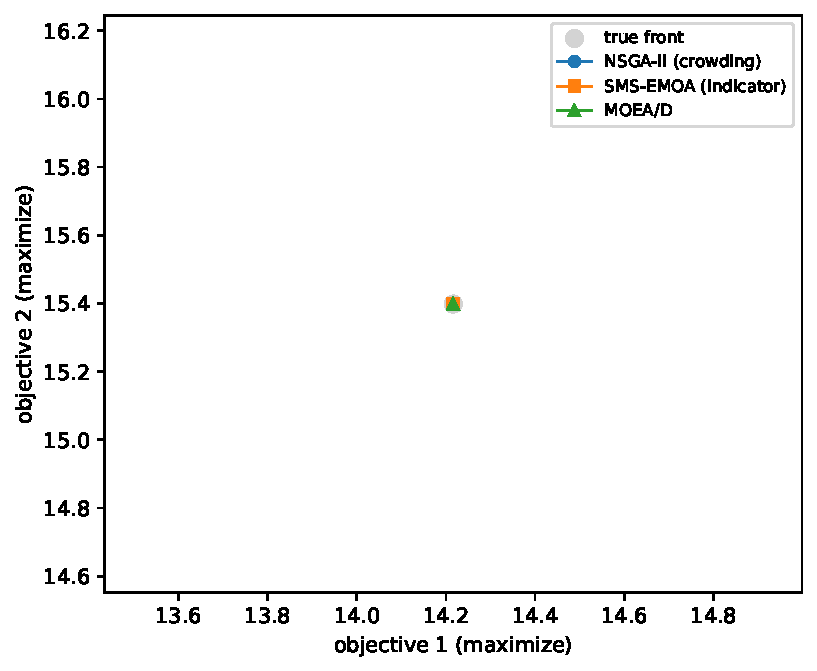
\includegraphics[width=0.72\textwidth]{fig_mo_comparison.pdf}
\caption{Approximation fronts obtained by the three multi-objective paradigms on
a bi-objective linear 0/1 problem, against the true Pareto front. All three
recover the front; hypervolume and IGD are reported by the accompanying example.}
\label{fig:mocomp}
\end{figure}

\subsection{Multi-Objective EDA Pipeline}

Below is a sketch of a multi-objective EDA using NSGA-II-style selection with a Bayesian network learner:

\begin{lstlisting}
from pateda.core.eda import EDA
from pateda.core.components import EDAComponents
from pateda.seeding.random_init import RandomInit
from pateda.selection.crowding import CrowdingDistanceSelection
from pateda.learning.ebna import LearnEBNA
from pateda.sampling.bayesian_network import SampleBayesianNetwork
from pateda.replacement.elitist import ElitistReplacement
from pateda.stop_conditions.max_generations import MaxGenerations
import numpy as np

n_vars, pop_size = 20, 500

def mo_func(x):
    f1 = np.sum(x)
    f2 = np.sum(1 - x)
    return np.array([f1, f2])

components = EDAComponents(
    seeding        = RandomInit(),
    selection      = CrowdingDistanceSelection(n_select=pop_size // 2),
    learning       = LearnEBNA(),
    sampling       = SampleBayesianNetwork(n_samples=pop_size),
    replacement    = ElitistReplacement(n_elite=1),
    stop_condition = MaxGenerations(50),
)
eda = EDA(pop_size, n_vars, mo_func,
          np.full(n_vars, 2), components)
stats, cache = eda.run()
\end{lstlisting}

\subsection{Extracting Pareto Fronts}

After running the EDA with \texttt{cache\_config} that stores populations and
fitness values, the full Pareto set approximation can be extracted:

\begin{lstlisting}
from pateda.selection.utils.pareto import find_pareto_set
import numpy as np

all_pop = np.vstack(cache.populations)
all_fit = np.vstack(cache.fitness_values)
pareto_idx = find_pareto_set(all_fit)   # indices of the non-dominated set
pareto_pop = all_pop[pareto_idx]
pareto_fit = all_fit[pareto_idx]
\end{lstlisting}

%% ============================================================
\section{Knowledge Extraction and Transfer Learning}
\label{sec:knowledge}
%% ============================================================

One of the most distinctive features of pateda---inherited from MATEDA-2.0---is the ability to extract and visualize knowledge from the probabilistic models learned during the EDA search.  The \texttt{knowledge\_extraction} module provides tools organized into the following categories.

\subsection{Dependency Analysis}

\texttt{knowledge\_extraction/dependency\_analysis.py} provides:

\begin{description}
  \item[\texttt{compute\_correlation\_matrix}]
    Computes the Pearson correlation matrix between variables from a population.

  \item[\texttt{learn\_bayesian\_network}]
    Learns a Bayesian network structure from a population using score-and-search.

  \item[\texttt{learn\_gaussian\_network}]
    Learns a Gaussian graphical model from continuous data.

  \item[\texttt{analyze\_variable\_dependencies}]
    Computes pairwise mutual information and tests for marginal independence.

  \item[\texttt{compute\_mutual\_information}]
    Mutual information between two discrete random variables.
\end{description}

\subsection{Fitness Measures}

\texttt{knowledge\_extraction/fitness\_measures.py} provides tools to
quantify the EDA's behavior over generations:

\begin{description}
  \item[Response to selection $R(t)$]
    $R(t) = \bar{f}(t+1) - \bar{f}(t)$: improvement in mean fitness
    from one generation to the next.

  \item[Amount of selection $S(t)$]
    $S(t) = \bar{f}_s(t) - \bar{f}(t)$: difference between the mean
    fitness of the selected subset and the whole population.

  \item[Realized heritability $b(t)$]
    $b(t) = R(t) / S(t)$: fraction of the selection differential that
    is realized in the next generation \citep{Muhlenbein:1997}.
\end{description}

\subsection{Network Measures and Visualizations}

For models based on graphs (Bayesian networks, Markov networks, trees),
pateda tracks which edges appear across generations and runs:

\begin{description}
  \item[\textbf{Edge frequency matrix}]
    \citep{Echegoyen_et_al:2007,Santana_et_al:2007b}.
    The $(i,j)$ entry counts how often the edge $(X_i, X_j)$ appeared
    in the structures learned across all runs and generations.  Bright
    colors in the heat-map indicate frequent structural relationships,
    often corresponding to true problem-structure interactions.

  \item[\textbf{Dendrogram of edges}]
    Hierarchical clustering of edges by co-occurrence frequency, displayed
    as a dendrogram \citep{Hauschild_and_Pelikan:2008}.

  \item[\textbf{Parallel coordinate view}]
    Each axis is a selected edge; each line connects edges that co-occur
    in the same structure at the same generation.

  \item[\textbf{Glyph representation}]
    A grid of glyphs (one per run $\times$ generation) showing which
    edges are present in each learned structure.
\end{description}

Scalar structural descriptors of the learned graphs --- degree distribution,
clustering coefficient, betweenness, motif counts, and their evolution --- are
computed in \texttt{knowledge\_extraction/network\_measures.py} and plotted by the
helpers in \texttt{network\_visualizations.py}
(\texttt{plot\_edge\_frequency\_matrix}, \texttt{plot\_measures\_evolution},
\texttt{plot\_network\_snapshots}, \texttt{plot\_degree\_distribution}). Because
\texttt{cache.models} stores the actual model learned at each generation
(Section~\ref{sec:eda}), all of these are produced from a single cached run.

Figures~\ref{fig:bnlearned}--\ref{fig:structevo} illustrate the workflow on a
concatenated order-3 deceptive function ($n=15$, five blocks of three variables)
optimized with EBNA. The single learned network (Figure~\ref{fig:bnlearned})
already recovers the true block structure: edges appear \emph{within} the trap
blocks and not across them. Accumulating the edges over all generations gives the
edge-frequency matrix of Figure~\ref{fig:edgefreq}, whose block-diagonal pattern
is a fingerprint of the problem's true interactions. Finally,
Figure~\ref{fig:structevo} shows how the structure emerges along the run.

\begin{figure}[ht]
\centering
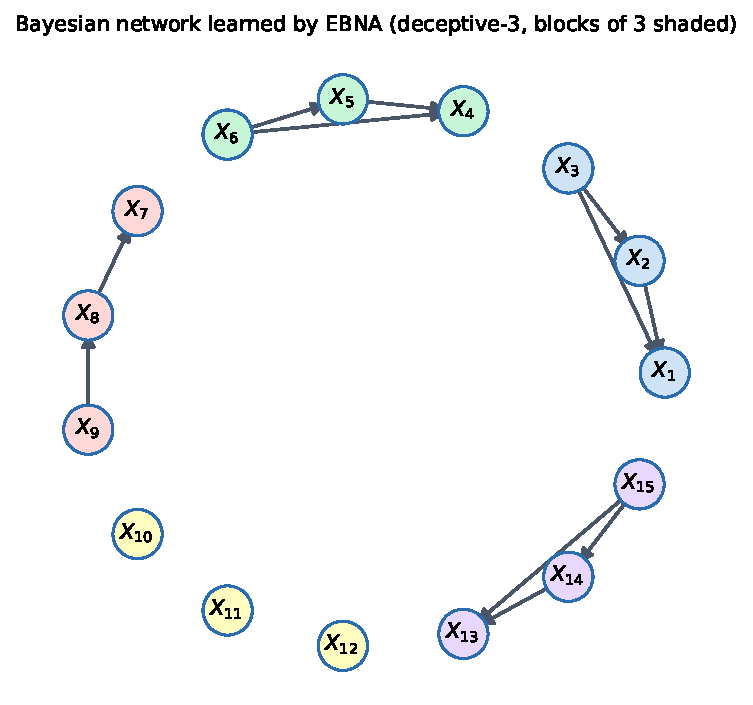
\includegraphics[width=0.62\textwidth]{fig_bn_learned.pdf}
\caption{A Bayesian network learned by EBNA on the deceptive-3 problem. Nodes are
shaded by their true order-3 block; the learned edges fall within blocks,
recovering the problem structure.}
\label{fig:bnlearned}
\end{figure}

\begin{figure}[ht]
\centering
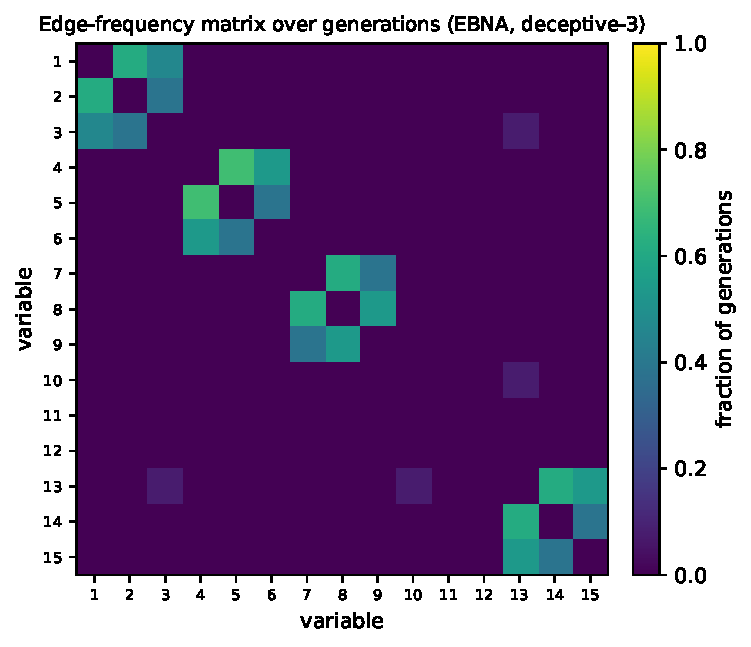
\includegraphics[width=0.55\textwidth]{fig_edge_frequency.pdf}
\caption{Edge-frequency matrix accumulated over generations for the same run. Each
entry is the fraction of generations in which the corresponding (undirected) edge
was present; the block-diagonal pattern matches the true interaction structure.}
\label{fig:edgefreq}
\end{figure}

\begin{figure}[ht]
\centering
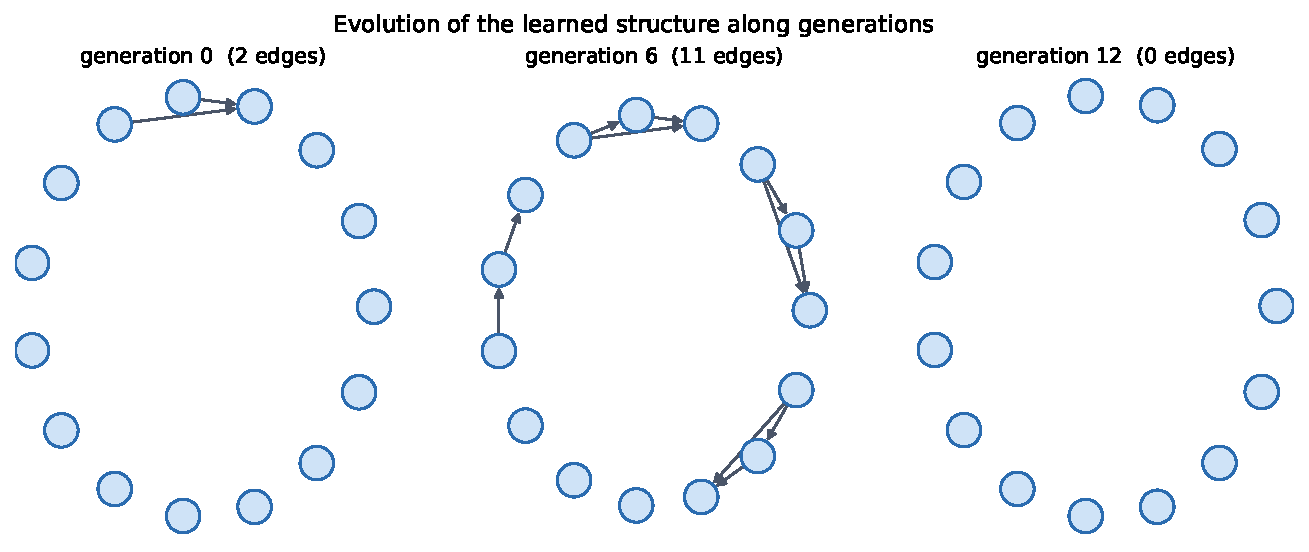
\includegraphics[width=\textwidth]{fig_structure_evolution.pdf}
\caption{Evolution of the learned structure along the run (early, middle, and late
generation). The model starts nearly empty and progressively concentrates edges
inside the deceptive blocks.}
\label{fig:structevo}
\end{figure}

\subsection{Continuous Variable Analysis}

For continuous EDAs, \texttt{knowledge\_extraction/continuous\_visualizations.py}
and \texttt{gaussian\_networks.py} provide tools to visualize the models learned
by Gaussian and Gaussian-network EDAs: \texttt{plot\_gaussian\_parameter\_evolution}
tracks the means, variances and correlations across generations;
\texttt{plot\_precision\_heatmap} and \texttt{plot\_partial\_correlation\_network}
display the sparse conditional-independence structure recovered by a
Gaussian-network (GMRF) EDA, where a zero in the precision matrix is a
conditional independence; and \texttt{plot\_network\_comparison} contrasts two
learned structures.

For copula-based EDAs, the vine model is not a single covariance matrix but a
\emph{cascade of trees}, each level pairing (conditional) variables through a
bivariate copula. The \texttt{vine\_analysis.py} module together with
\texttt{plot\_vine\_first\_tree}, \texttt{plot\_family\_composition},
\texttt{plot\_tau\_by\_tree} and \texttt{plot\_vine\_evolution} visualize this
regular-vine decomposition: which pairs are linked at each tree level, which
copula family (Gaussian, Clayton, Gumbel, \ldots) was selected for each edge, and
the strength of dependence (Kendall's~$\tau$) per tree.
Figure~\ref{fig:vine} shows the schematic structure of a regular vine over five
variables.

\begin{figure}[ht]
\centering
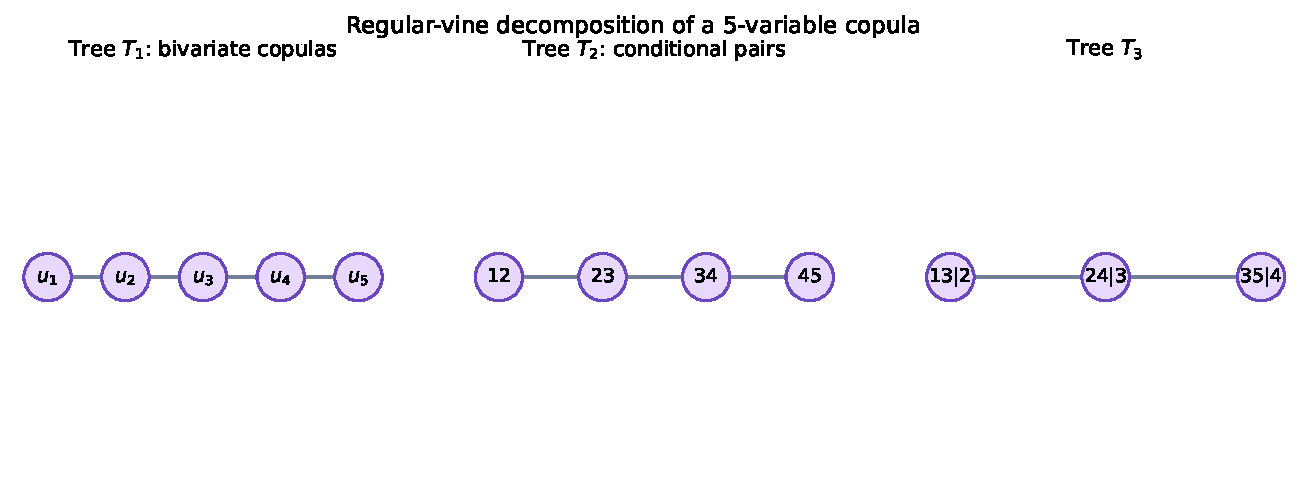
\includegraphics[width=\textwidth]{fig_vine_structure.pdf}
\caption{Regular-vine (R-vine) decomposition of a 5-variable copula. Tree $T_1$
pairs the variables through unconditional bivariate copulas; each subsequent tree
$T_k$ has the edges of $T_{k-1}$ as its nodes and models conditional pairs (e.g.
$13\mid 2$), so the full joint density factorizes into a product of bivariate
copulas.}
\label{fig:vine}
\end{figure}

\subsection{Transfer Learning}
\label{sec:transfer}

The knowledge an EDA extracts about the structure of a problem need not be
discarded when the run ends: it can be \emph{transferred} to accelerate the
solution of related problems. Transfer learning is attractive for EDAs precisely
because they already build an explicit, inspectable model of the search
distribution --- the same edge-frequency and interaction information used for
knowledge extraction above is exactly what a new run can be biased with. It is
especially valuable when many similar instances must be solved (e.g. the same
combinatorial problem over changing data) or when fitness evaluations are
expensive and a warm start pays off \citep{Santana_et_al:2012transfer,Hauschild_and_Pelikan:2012}.

Following \citet{Santana_et_al:2012transfer,Hauschild_and_Pelikan:2012}, three
kinds of transfer are relevant to EDAs:
\begin{description}
  \item[Structural transfer] Reuse of the learned \emph{dependency structure}:
    the aggregated interaction/edge-frequency matrix of a source run becomes an
    a-priori \texttt{interaction\_matrix} that restricts (or biases) structure
    learning in the target run --- exactly the restriction mechanism used by
    \texttt{TreeEDAR}, \texttt{MNFDAR} and \texttt{MNFDAGR}
    (Section~\ref{sec:apriori}). This is the form validated on multi-marker
    tagging-SNP selection by \citet{Santana_et_al:2012transfer}.
  \item[Parametric transfer] Reuse of \emph{parameters/solutions}: seeding the
    target population from the source's best solutions or MPEs
    (\texttt{SeedThisPop}), i.e. a warm start.
  \item[Bias transfer] A \emph{soft} distance-based bias on the structure score
    that favours short-range dependencies learned to be useful on the source
    problem, as in the soft distance-based bias of \citet{Hauschild_and_Pelikan:2012}.
\end{description}
These forms of transfer are supported by the \texttt{knowledge\_extraction.transfer}
module. \texttt{aggregate\_edge\_frequencies(cache.models)} averages the linkage
graphs learned across a source run into an edge-frequency matrix;
\texttt{structure\_to\_interaction\_matrix(freq, threshold)} thresholds it into a
binary \texttt{interaction\_matrix} for hard structural transfer into
\texttt{TreeEDAR}/\texttt{MNFDAR}/\texttt{MNFDAGR}. The \texttt{TransferredStructure}
container packages this information, can \texttt{save}/\texttt{load} it to disk
(so structure learned on one problem is reused on another), and exposes a
\texttt{soft\_bias()} edge prior for the soft-bias variant. Finally,
\texttt{warm\_start\_population(...)} builds a warm-start population from a source
run's best solutions for parametric transfer via \texttt{SeedThisPop}.

\begin{lstlisting}
from pateda.knowledge_extraction.transfer import TransferredStructure
ts = TransferredStructure.from_models(source_cache.models)   # aggregate + persist
ts.save("problemA_structure.npz")
# ... later, on a related problem B:
M = TransferredStructure.load("problemA_structure.npz").interaction_matrix(0.5)
alg = TreeEDAR(n_vars=n, cardinality=2, fitness_func=fB, interaction_matrix=M)
\end{lstlisting}

%% ============================================================
\section{Injecting A-Priori Knowledge}
\label{sec:apriori}
%% ============================================================

A key advantage of EDA-based approaches is that a-priori information about
the problem structure can be directly incorporated into the model, potentially
reducing the search space and accelerating convergence
\citep{Santana_et_al:2009b}. Because an EDA's model \emph{is} the search bias,
partial knowledge of the problem --- which variables interact, which values are
plausible, which configurations are feasible --- can be injected exactly where it
matters instead of being encoded indirectly in operators. Restricting structure
learning to a known interaction graph removes spurious edges that small
selected sets would otherwise induce, and has been shown to improve both model
quality and search on structured problems such as protein-structure prediction,
side-chain placement and tagging-SNP selection
\citep{Santana_et_al:2007b,Santana_et_al:2009b,Santana_et_al:2012transfer}. The
mechanisms below --- fixed factorizations, interaction matrices, biased
initialization, and hard constraints --- are the concrete entry points.
Figure~\ref{fig:apriori} illustrates the interaction-matrix mechanism.

\begin{figure}[ht]
\centering
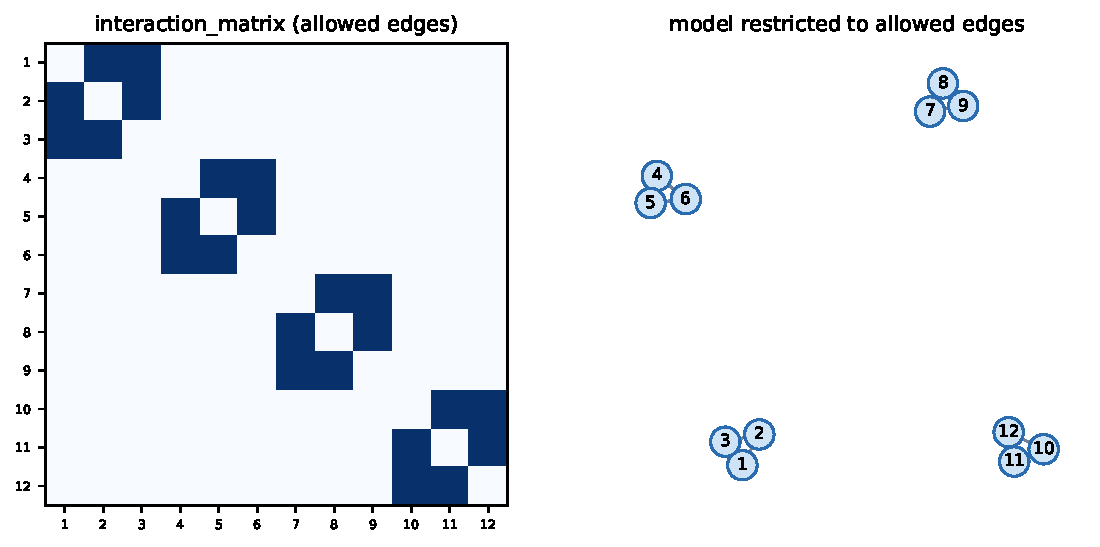
\includegraphics[width=0.85\textwidth]{fig_apriori_interaction.pdf}
\caption{A-priori structural information as an interaction matrix. A binary
matrix (left) lists the variable pairs allowed to interact; the restricted EDAs
(\texttt{TreeEDAR}, \texttt{MNFDAR}, \texttt{MNFDAGR}) learn a model only over
those edges (right), here a block-diagonal structure matching an additively
decomposable problem.}
\label{fig:apriori}
\end{figure}

\subsection{Fixed Factorizations}

When the structure of the optimal model is known a priori (e.g., from domain
knowledge or problem decomposition), the user can supply a fixed clique
structure to \texttt{FDA}:

\begin{lstlisting}
import numpy as np
from pateda import FDA

# Fixed Markov-chain structure for a 10-variable problem
n = 10
cliques = np.array([
    [0, 1, 0],       # factor 1: only X_1
    [1, 1, 0, 1],    # factor 2: X_1 | X_2
    [1, 1, 1, 2],    # factor 3: X_2 | X_3
    # ... etc.
])

alg = FDA(n_vars=n, cardinality=2,
          fitness_func=my_func,
          cliques=cliques,
          pop_size=300, n_gen=50)
stats, _ = alg.run()
\end{lstlisting}

The Markov-chain FDA with order 1 is the natural model for problems with
sequential structure, such as the HP protein folding model
\citep{Dill:1985,Santana_et_al:2004}.

\subsection{Interaction Matrices}

\texttt{TreeEDAR}, \texttt{MNFDAR}, and \texttt{MNFDAGR} accept an
\texttt{interaction\_matrix} parameter: an $n \times n$ binary matrix where
entry $(i,j)=1$ means that variables $X_i$ and $X_j$ may be connected in
the learned model, and $(i,j)=0$ forbids the connection.  This allows the
user to encode known independence relationships or restrict the model to
biologically or physically plausible interactions.

\subsection{Biased Initialization}

\texttt{BiasInit} seeds the initial population with variable-wise biases.
For example, if domain knowledge indicates that variable $X_5$ is likely to
take value 1 in good solutions, a higher prior probability can be assigned:

\begin{lstlisting}
from pateda.seeding.bias_init import BiasInit

seeder = BiasInit(probs=np.array([0.5]*20 + [0.9]))
# Variable 21 is initialized with P(X=1) = 0.9
\end{lstlisting}

\subsection{Constrained Search}

Most real optimization problems are \emph{constrained}: only a subset of the
representable strings are feasible. This is awkward for EDAs specifically because
the model is learned from data and then sampled independently variable by
variable: even if every selected (feasible) parent satisfies a global constraint,
probabilistic logic sampling recombines their marginals and readily produces
infeasible offspring. The three generic remedies --- penalizing infeasibility in
the fitness, repairing sampled solutions (Section on repairing methods), or
building feasibility into the sampler --- all apply in \texttt{pateda}; the third
is the most reliable when it can be arranged.

A particularly clean case is the \emph{unitation constraint}, which fixes the
number of ones (the \emph{unitation} $u(\mathbf{x})=\sum_i x_i$) of every binary
solution to a constant $k$. It appears whenever exactly $k$ items must be chosen:
feature selection with a fixed budget, fixed-size subset problems, balanced
assignments. The feasible region is the set of length-$n$ binary strings with
exactly $k$ ones, and independent univariate sampling almost never lands in it.

\texttt{pateda} provides two simple constraint-preserving EDAs for this case:

\begin{description}
  \item[\texttt{CUMDA}] \citep{Santana_and_Ochoa:1999b}.
    Constrained UMDA. It learns univariate marginals as usual but \emph{samples}
    with a scheme (stochastic universal sampling over the marginals) that emits
    exactly $k$ ones per solution, so feasibility is maintained by construction;
    the seeding method likewise produces only feasible initial solutions.
  \item[\texttt{CFDA}] \citep{Santana_et_al:2001c}.
    Constrained FDA. Same fixed-unitation guarantee, but over a tree-structured
    factorized model rather than independent marginals, so it can additionally
    capture pairwise dependencies among the chosen positions.
\end{description}

Both are ``simple'' in the sense that they handle one specific, if common, family
of constraints exactly; general constraints still require penalties or repair.

The weighting of selected solutions during model learning --- another way of
injecting fitness information into the model --- is discussed with the learning
machinery in Section~\ref{sec:weighted_learning}.



\section{Extensions to pateda}
\label{sec:extensions}

The component architecture of \texttt{pateda} was designed to be extended. Three
specialized libraries take \texttt{pateda} as a dependency and reuse its
executor, components, and statistics/knowledge machinery while replacing the
representation or the model family. They are distributed separately so that their
heavier dependencies (e.g. permutation-specific code, PyTorch) do not burden the
core library.

\subsection{Problems with permutation representation (\texttt{perm\_pateda})}

\texttt{perm\_pateda}\footnote{\url{https://github.com/rsantana-isg/perm_pateda}}
targets optimization problems whose solutions are \emph{permutations} (the
travelling salesman problem, the linear ordering problem, flowshop scheduling,
QAP). Permutations cannot be modelled variable-by-variable as integer vectors
without producing infeasible offspring, so \texttt{perm\_pateda} supplies
permutation-specific learning and sampling components --- distance-based
probability models such as Mallows and generalized-Mallows models, and models
based on the Plackett--Luce and factoradic representations --- together with
permutation seeding, repair, and benchmark problems. Everything else (the EDA
loop, selection, replacement, stopping, statistics) is inherited from
\texttt{pateda}.

\subsection{Model learning with neural networks (\texttt{nn\_pateda})}

\texttt{nn\_pateda}\footnote{\url{https://github.com/rsantana-isg/nn_pateda}}
replaces the probabilistic graphical model at the core of an EDA by a
\emph{neural} density/generative model. It provides learning/sampling components
built on autoencoders and variational autoencoders, generative adversarial
networks, and denoising/`backdrive' models that map fitness gradients back onto
solutions \citep{Garciarena_et_al:2018a,Marti_et_al:2008}. These plug into the
same \texttt{learning}/\texttt{sampling} slots as the classical learners, so a
neural EDA is assembled exactly like a UMDA or EBNA; PyTorch is used for the
network components (with GPU support when available).

\subsection{Searching in the neural latent representation space (\texttt{latent\_search})}

\texttt{latent\_search}\footnote{\url{https://github.com/rsantana-isg/latent_search}}
implements search algorithms that first \emph{learn a latent representation} of
the optimization problem --- typically with an autoencoder trained on good
solutions --- and then perform the search in that lower-dimensional, smoother
latent space, decoding candidates back to the original space for evaluation. This
``deep optimization'' idea lets the algorithm discover and reuse building blocks
captured by the representation, and connects EDAs to representation-learning
approaches to black-box optimization.

%% ============================================================
\section{EDA Pipelines: model operators and a generative grammar}
\label{sec:pipelines}

An \emph{EDA pipeline} is a consistent assembly of EDA components --- seeding, selection, learning, sampling, replacement, optional local search and mutation, and a stopping condition --- that together define a working EDA.  The module \texttt{pateda.pipelines} adds two ingredients that make the space of pipelines both richer and searchable.

\subsection{Model operators: MODMOD and MODCONV}

Beyond the primary components of Section~\ref{sec:components}, two families of operators transform a learned probabilistic model (its graph \emph{and} its tables):

\begin{description}
  \item[MODMOD (model modifier)] takes a model and returns a new model, usually simpler:
    \texttt{prune\_factorized} reduces every clique of a factorized / junction model to at most $K$ variables by marginalizing the dropped ones out of the factors;
    \texttt{tree\_to\_forest} cuts the weakest tree edges into a forest;
    \texttt{tree\_to\_malign} keeps only the \emph{malign} edges (those whose interaction changes the conditional mode), a model-level Tree-EDA-M.
  \item[MODCONV (model conversor)] changes the model \emph{type} so a different sampler can consume it:
    \texttt{bn\_to\_factorized} turns a Bayesian network into an equivalent factorized model (one conditional clique per variable, in ancestral order), which the factorized samplers (\texttt{SampleFDA}, \texttt{SampleGibbs}) can sample.
\end{description}

The operator ``$\mathrm{LM}\ \mathrm{MODCONV}\ \mathrm{SM}$'' of the design is realized by wrapping a learner in \texttt{ModifiedLearning(LM, [operators])}: the wrapper runs the base learner and applies the operator chain to its model, so that the resulting model \texttt{NLM} is samplable by \texttt{SM}.  Every operator is robust (returns the model unchanged when inapplicable), so a modifier never breaks a pipeline.  These operators substantially increase the number of feasible learning/sampling combinations: for example every Bayesian-network learner (EBNA, BOA, hBOA, LFDA, PADA) can now feed the factorized samplers.

\subsection{A context-free grammar for feasible pipelines}

Following the grammar-based AutoML literature \citep{deSa_et_al:2017,Marinescu_et_al:2021}, \texttt{pateda.pipelines.grammar} defines a context-free grammar whose language is the set of valid discrete-EDA pipelines.  The model part is organized into \emph{typed blocks} (one per model type), so that a learner is always paired with a compatible sampler --- directly, or through a MODCONV.  A random derivation of the grammar is a flat list of terminals (each carrying a role and a factory) that \texttt{build\_pipeline} reassembles into an \texttt{EDA}.

The top of the grammar is (``$|$'' denotes choice, capitalized names are
non-terminals):

\begin{lstlisting}[language=]
Pipeline   -> Seeding Selection ModelBlock Replacement LocalOpt Mutation Stop
ModelBlock -> FacBlock | BNBlock | MarkovNetBlock | IntFDABlock
            | RegMarkovBlock | MarkovChainBlock
FacBlock   -> FacLearner FacModMod SampleFDA
BNBlock    -> BNLearner ( SampleBN | bn_to_factorized FacModMod SampleFDA )
FacModMod  -> empty | prune_factorized | tree_to_forest | tree_to_malign
\end{lstlisting}

The typed \texttt{ModelBlock} is the key to feasibility: each block pairs a family
of learners with a sampler that can consume their model, and the optional model
operators (\texttt{FacModMod}, and the \texttt{bn\_to\_factorized} MODCONV in
\texttt{BNBlock}) are the bridges introduced above. Consequently \emph{every}
complete derivation is type-consistent by construction --- a learner is never
paired with an incompatible sampler. The residual fraction of random pipelines
that still fail at run time comes only from data/representation edge cases
(a binary-only mutation applied to a non-binary problem, a learner starved by a
tiny population), which the accompanying demo measures explicitly rather than
hiding.

The grammar's generality is measured by the fraction of pateda's discrete-EDA component implementations it can emit (per category: selection, learning, sampling, local optimization, mutation, replacement, \ldots), and its practicality by the fraction of randomly sampled pipelines that run without error; both are reported by the accompanying example.

\subsection{A multi-objective meta-optimizer over pipelines}

\texttt{PipelineMetaOptimizer} searches the space of pipelines defined by the grammar with a grammar-guided genetic algorithm.  Each candidate is a whole pipeline, evaluated by building it and running it on a target problem at a \emph{fixed inner budget} (population size and number of generations); this yields two conflicting objectives --- the best objective value reached (to maximize) and the wall-clock time spent (to minimize).  Because these objectives trade off, the search uses NSGA-II selection \citep{Deb_et_al:2002} and returns the \emph{Pareto set} of pipelines, from the cheap-but-weaker to the strong-but-slower, rather than a single winner.  The genetic operators respect the grammar: crossover swaps whole slots between parents --- selection, replacement, local search, mutation, and the model block (learner $+$ model operators $+$ sampler) as a unit --- and mutation re-derives one slot, so every offspring stays type-consistent.  On a difficult, fully deceptive problem (a concatenated trap-5, where univariate models are fast but stall and linkage-learning models are slower but succeed) the meta-optimizer recovers the whole quality/time trade-off automatically, letting a practitioner pick the pipeline at the knee of the front for their time budget.

%% ============================================================
\section{Conclusions}
%% ============================================================

\texttt{pateda} is a comprehensive Python library for estimation of distribution
algorithms over discrete and continuous, single- and multi-objective search
spaces. It combines a set of plug-and-play algorithm classes with a fully modular
component architecture --- seeding, selection, learning, sampling, replacement,
mutation, crossover, local optimization, and repairing are independently
swappable --- and a knowledge-extraction module that turns the models learned
during search into analyzable, visualizable descriptions of problem structure.

While retaining the modular philosophy of \texttt{MATEDA-2.0}, this version
introduces a set of developments that go beyond it:

\begin{itemize}
  \item support for discrete problems with heterogeneous (binary and non-binary)
    variable cardinalities;
  \item model learning that can explicitly use selection probabilities to weight
    solutions (Section~\ref{sec:weighted_learning}), subsuming earlier
    fitness-weighted schemes;
  \item injection of a-priori problem-structure information, and its reuse across
    problems through transfer learning (Sections~\ref{sec:apriori}
    and~\ref{sec:transfer});
  \item an automatic EDA-pipeline search built on model operators (MODMOD /
    MODCONV) and a context-free grammar of feasible pipelines
    (Section~\ref{sec:pipelines});
  \item sampling based on the most probable configurations of the learned model
    (Section~\ref{sec:mpe});
  \item a dedicated Bayesian-network learning library (\texttt{bayes\_nets}) with
    a broad set of structure-learning algorithms, vine-copula models for
    continuous problems, and mixture models for discrete and continuous problems;
  \item three derived libraries --- \texttt{perm\_pateda}, \texttt{nn\_pateda} and
    \texttt{latent\_search} (Section~\ref{sec:extensions}) --- that extend the
    framework to permutation problems, neural-network models, and search in
    learned latent spaces.
\end{itemize}

The developments collected in \texttt{ROADMAP\_New\_Functs.md} have been
implemented in this version: diversity-preserving replacement schemes (crowding,
restricted tournament, clustering), convergence- and stagnation-based stopping
conditions, generalized probabilistic seeding, multi-objective metric tracking
with a worked variant comparison, a continuous memetic example, and a
first-class structural transfer-learning API. Further work will broaden the
continuous-EDA family and add larger multi-objective and real-world benchmarks.

%% ============================================================
\bibliographystyle{abbrv}
\bibliography{pateda}
%% ============================================================

\end{document}
